%Document styles, font text, sizes
\documentclass[12pt, journal, transmag, onecolumn]{IEEEtran}   	% use "amsart" instead of "article" for AMSLaTeX format

%LaTeX packages to be used:
\usepackage{graphicx}				
\usepackage{blindtext}
\usepackage{amssymb}
\usepackage{setspace}
\usepackage{hyperref}
\usepackage{subcaption}
\usepackage{mathtools}
\usepackage{multirow}
\usepackage{tabularx}
\usepackage[normalem]{ulem}\usepackage[final]{pdfpages}
\useunder{\uline}{\ul}{}
\DeclarePairedDelimiter\ceil{\lceil}{\rceil}
\DeclarePairedDelimiter\floor{\lfloor}{\rfloor}




%Document begins here. Separate sections are written in separate .tex files and inputted into the main .tex file
\begin{document}
\title{Cost Effective Demonstration of Wave-Particle\\ Duality on a Table Top}
\author{\IEEEauthorblockN{Johnny Allain-Labon, Chong Keat Gea, Steven Vuong, Georges Ajaka, \\Benji Berczi, Kelvin Fang, Alex Stock, Mohit Motwani}
\IEEEauthorblockA{11/1/18, Lab 1, Department of Physics and Astronomy, University College London, London WC1E 6BT
\\Board member: Professor Ryan Nichol}%
}


\IEEEtitleabstractindextext{%
\begin{abstract}

\blindtext

\end{abstract}
}

% make the title area
\maketitle
\clearpage
\tableofcontents

\clearpage
\spacing{1.2}
\section{Introduction (MM)}
An age-old and much investigated field of research in science has been the nature of light. For centuries, scientists have endeavoured to understand its nature and fundamental properties. At the turn of the 20th century, light was widely believed to behave as a wave, but the discovery of phenomena such as the photoelectric effect called this theory into question. Eventually, it was agreed that light exhibited both wave-like and particle-like behaviour, a phenomenon known as wave-particle duality. The interpretation of this quantum mechanical behaviour, however, is still open to debate.

The commonly accepted interpretation, known as the Copenhagen Interpretation, was first proposed by Niels Bohr and Werner Heisenberg in 1927. It pushed forward the idea that a physical system would only have definite properties upon measurement; prior to measurement it was only possible to measure probabilities of obtaining a given measurement. An alternative interpretation, the De Broglie –- Bohm theory, was pushed forwards in 1952. It is deterministic in nature: it claims that even prior to observation there exists a driving equation or `pilot wave' whose properties determine measurements. In 2005, research suggested \cite{couder} that droplets bouncing on a surface could display quantum mechanical behaviour as proposed by pilot wave theory. Indeed, this macroscopic system was a remarkably good analogy for the pilot wave theory; waves induced by a driving droplet quite closely match a driving wave-equation determining the results of measurements. 
\subsection{Aims}\todo{check to see if matches summary}
To this end, the purpose of this project was to develop a cost-effective table top version of the experiment used by \textit{Couder et al.}, demonstrating the various different behaviours of bouncing droplets. Such motion could include simple oscillations, motion parallel to the liquid surface and double slit diffraction of droplet generated waves. It was intended to be paired with a computer based visualisation that can display effects outside the bounds of this apparatus. The overarching goal was to develop a prototype that can be used for outreach purposes, allowing  students to the grasp the non-intuitive nature of quantum mechanics. 

\subsection{Objectives}
The above aims raised the following core project objectives: 
\begin{enumerate}
   \item Development of table top apparatus: 
   \begin{enumerate}
     \item To create a working prototype capable of displaying basic  motion, such as bouncing and walking droplets.
     \item To obtain high speed cameras capable of recording droplet motion
     \item To further improve the prototype, and demonstrate multiple droplet motion (such as droplets repelling and coalescing) and phenomena such as double slit diffraction
    \end{enumerate}
   \item Development of an in-depth simulation:
   \begin{enumerate}
    \item To identify a suitable programming language for simulation purposes
     \item To implement required code in chosen language in order to display droplet motion.
     \item To extend the capabilities of the program in order to cover aspects of quantum mechanics not displayable by the experimental apparatus. Such effects may include double slit diffraction and tunnelling effects, where the droplet escapes through the barrier of a potential well.
    \end{enumerate}
    \item Creating an iteration of the initial prototype usable in college/undergraduate courses as a demonstration tool.  
   \begin{enumerate}
     \item To create a standalone version of the simulation program.
     \item To create a simple to use version of the experimental. apparatus, for third-party users.
     \item To write a business plan for implementation in future.
     \item To explore the possibility of testing the apparatus with undergraduates and A-level students.
    \end{enumerate}
\end{enumerate}


\section{Theory (MM, AS)}\label{theory}
\subsection{Droplet motion}
This investigation focuses on the motion of moving droplets on a liquid surface. In 1978 it was reported \cite{Walker} that droplets vibrating at a certain frequency upon a soap-solution surface would not immediately coalesce, but could maintain motion for up to 18 minutes. Couder \textit{et al.} further researched this phenomenon in 2005 \cite{couder}. Using a silicon oil surface (with no soap-substrate) they discovered that it was possible to create a   an oscillating droplet at certain frequencies, and even walking droplets that moved parallel to the surface. 
The walking droplets were created by simply vibrating the liquid surface vertically at a frequency determined by: (\ref{eq:bouncing regime condition}):

\begin{equation} \label{eq:bouncing regime condition}
\frac{\gamma_{m}^{B}}{g}\approx 1
\end{equation}
$g$ is the acceleration due to gravity, $\gamma_{m}^{B}$ is the specific value of co-efficient $\gamma_{m}$ of (\ref{eq:vertical acceleration}).


\begin{equation} \label{eq:vertical acceleration}
\gamma=\gamma_{m}cos(2 \pi f_0t) 
\end{equation}

(\ref{eq:vertical acceleration}) determines $\gamma$, which is the vertical acceleration of the fluid, $f_0$ is the driving frequency of the liquid and $t$ is time. The droplets bounce due to a remarkably simple mechanism. Upon collision of a droplet with the liquid, there exists a thin layer of air trapped between the two surfaces. Normally, the droplet will coalesce with a surface in a matter of seconds, as this air is forced away. However above a threshold value of $\gamma_{m}$, the droplet will instead bounce, as the air film retains its integrity, forcing the droplet upwards. By specifying a threshold vertical acceleration, it is also ensured that the air film will have a chance to replenish after each subsequent bounce, allowing the motion to be periodic over a large period of time. The regimes in which different types of motion occur are described in Figure \ref{regimes}.

\begin{figure}[ht]
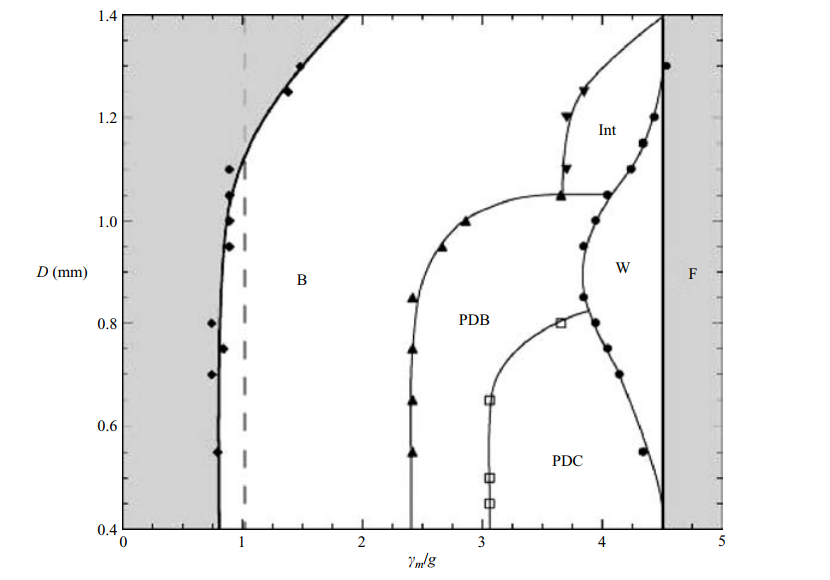
\includegraphics[width=12cm]{theory/regime}
\centering
\caption{A graph of droplet diameter against $\frac{\gamma_{m}}{g}$ for an oscillating droplet in a vibrating liquid. It illustrates the different vertical acceleration regimes: Bouncing (B), Walking (W), Faraday instability (F), Period Doubling (PDB), transition from Periodic to chaotic behaviour (PDC)  and Intermittent behaviour (Int).}
\centering
\label{regimes}
\end{figure}

Furthermore, droplets can also exhibit motion parallel to the droplet surface. Such droplets are labelled walkers, and like bouncing droplets, they exist in a certain $\frac{\gamma_{m}}{g}$ regime, just below the onset of the Faraday instability. The Faraday instability is defined as the point at which a surface becomes spontaneously wavy. Just before its onset, a bouncing droplet has a period of motion twice that of its driving oscillation. It thus generates a damped travelling Faraday wave at each bounce, where Faraday waves are standing waves generated by a vibrating liquid. The subsequent landing then occurs on the reverse slope of this previously generated Faraday wave. This landing generates another travelling Faraday wave, and causes the droplet to perform a parabolic bounce, causing motion parallel to the surface. An intuitive way to understand this motion is to imagine jumping on a trampoline. Each time you land on the trampoline, a wave is generated. If you land again anywhere but at the centre of this wave, you spring off again, and your motion has a slight horizontal component, allowing you to travel around the trampoline. As the wave you generate when landing travels, you constantly land on its side, therefore there is a constant horizontal motion, allowing you to 'walk' around the trampoline. This motion is illustrated in Figure \ref{walker}. 

\begin{figure}[ht]
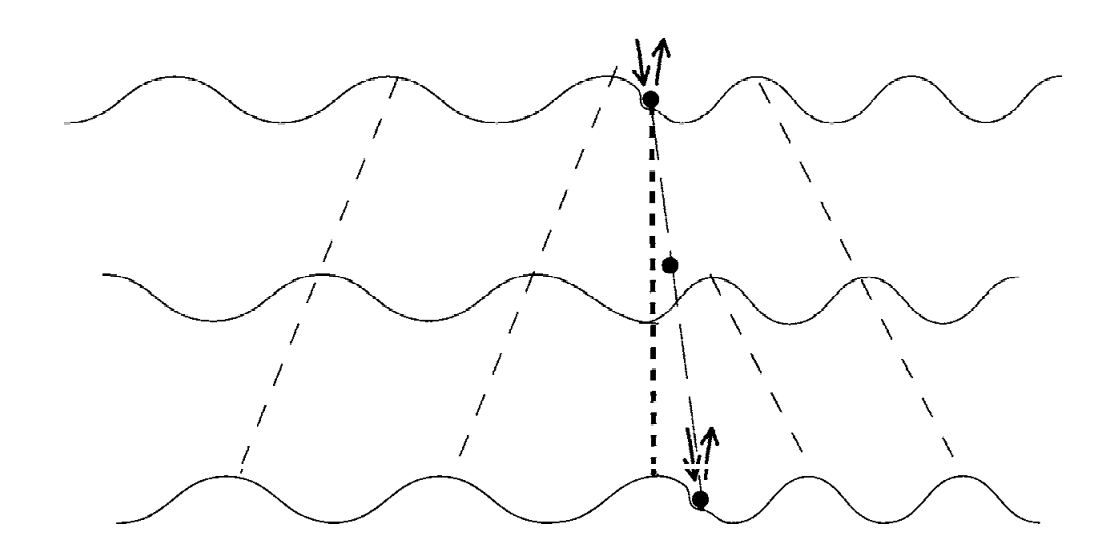
\includegraphics[width=12cm]{theory/walkingDroplet}
\centering
\caption{An illustration of a walking droplet's motion for subsequent bounces. The movement of droplet is exaggerated for visual purposes. In reality, wave amplitude decays with distance from droplet and is not necessarily constant; it is modulated by the driving force. }
\centering
\label{walker}

\end{figure}

Equations of motion for this droplet motion described above were taken from \cite{oza2013trajectory}, which showed that the surface wave produced on the $\textrm{n}^{\textrm{th}}$ impact of a particle at position $r_n$ and time $T_n$ on a surface oscillating vertically at $\omega$ above the Faraday threshold is given by (\ref{equ:heightSurfaceWave}). Here, $ h(\vec{r} , t)$ is the height of the wave at $\vec{r}$, $J_0$ is a Bessel function of the first kind, and wave number $k$ satisfies the relation $ J_0 \left( k \vec{r_0} \right) = 0$. $\vec{r_0}$ is a numerical cutoff parameter, while the amplitude of the wave, A is material specific and determined by the system parameters used. The exponential decay term at the end of the equation describes the wave decaying over time at a rate determined by the memory $Me$ and period of particle $T_f$.

\begin{equation}
h_n(\vec{r} , t) = A J_o\left(k\left|\vec{r} - \vec{r_n}\right| \right) e^{-\frac{\left(t-T_n\right)}{T_f Me}}
\label{equ:heightSurfaceWave}
\end{equation}

The overall surface wave can thus be described by the sum of all waves produced by every prior impact. Assuming the particle only interacts with the surface once every period (when the particle is at its lowest point), the overall wave equation $h (\vec{x} , t)$ is thus given by (\ref{equ:heightSumSurfaceWaves}).

\begin{equation}
h(\vec{r} , t) = \sum_{n=-\infty}^{\frac{t}{T_f}} A J_o\left(k\left|\vec{r} - \vec{r_n}\right| \right) e^{-\frac{\left(t-n T_f\right)}{T_f\times Me}}
\label{equ:heightSumSurfaceWaves}
\end{equation}

Furthermore, we know that the surface wave needs to consider relativistic effects. The coordinate transform on the wave formed by the $n^{\textrm{th}}$ impact of a particle at some velocity v is as follows:
\begin{equation}
h_n(\vec{r} , t) = A_0 cos\left(\omega_0 t - \frac{\gamma^2 \omega_0 v}{c^2}\right) J_0\left(k \left| \left(\vec{r} - \vec{r_n}\right)^{\prime \prime}  \right| \right)e^{-\frac{\left(t-n T_f\right)}{T_f\times Me}}
\end{equation}

Where:
\begin{equation}
\gamma = \frac{1}{\sqrt{1-\frac{v^2}{c^2}}}
\end{equation}
\begin{equation}
\left(\vec{r} - \vec{r_n}\right)^{\prime \prime} = \gamma^2(\vec{r_v}-\vec{v}t)+\gamma\vec{r_{\perp}}
\end{equation}

$\vec{r_v}$ and $\vec{r_{\perp}}$ are the components of $\left(\vec{r} - \vec{r_n}\right)$ in the direction of velocity and perpendicular to velocity respectively.

\subsection{The memory parameter $Me$}
The memory parameter,  $Me$ , represents the decay time of a wave produced from a given impact in terms of the time between each impact. It is defined by the ratio between the non-dimensional damping time $\tau$, and the Faraday period of the system $T_f$.
A droplet entering a walking state is a direct result of this memory parameter and can seen by the comparison of the high and low memory regimes \cite{couder11}.
In the high memory regime, the waves decay slowly, and so waves created in the distant past can still strongly influence the particle trajectory. However, in the low memory regime, the waves decay rapidly, so only waves created in the recent past can significantly influence the particle's trajectory. 


\todo{Subsection on multiple droplet interaction}
\subsection{May need section on interaction between multiple droplets if we use that data}
\todo{Fluid dynamics stuff}
\subsection{Fluid Dynamics}
If the height of the oil is known for the entire surface, the trajectory after a bounce at any point can be calculated using basic equations of motion. On collision, the impulse received by the droplet is found to be proportional to the gradient of the surface. This can then be used to find the velocity until the next collision. 
\spacing{1.2}

\clearpage
\section{Initial Apparatus}
The initial version of this apparatus is based  off previous run experiments by \textit{Harris et al.}. It consists of a 250 W, 8 Ohm High Powered Woofer With Aramid Fibre Cone, serving as the source of vibrations, mounted in a custom made ply-wood frame. The speakers volume, and thus the amplitude of the vibrations was altered through either a a signal generator or a signal generating app on a phone. In order to ensure that vibration amplitude was sufficiently large, an amplifier \todo{amplifier type}[] was used. This amplifier also allowed for bass and treble modification. 

A piece of plywood with a 6.5 inch diameter, that fit perfectly on the rim of the speaker.Graph paper was then cut into shape and placed on the wooden surface. The graph paper was attached to the wood surface using double sided tape. The wood surface was secured to the speaker using a combination of fold-back clips and double sided tape. A \todo{petri size}[] inch petri dish was filled with 50 cSt silicon oil. The petri dish was attached to the graph paper using double sided tape carefully placed on the edges of the dish, to ensure that the remains of tape did not coat its lower surface, which interfered with images. The droplet motion was observed using a high-speed camera capable of recording at 1,000 fps; the recording area was illuminated using two spotlights. 

\subsection{Box creation}
\todo{details on box creation from Gea}
To be filled in with the help of Gea.\\ 


\subsection{Droplet Creation}
A key aspect of this experiment involves creating a droplet of consistent size, in order to allow for various behavioural regimes to be consistently recreated. While previous such experiments use a 'trial-and-error' approach to such matters, due to our lack or ready access to strong light sources and suitable cameras, a more consistent approach was necessary.

An initial attempt was made using a needle, or segment of wire,  dipped this rapidly into the liquid surface. As this approach was unsuccessful,  an attempt was made to flick the top of the surface with the tool tip; a semi-reliable way of creating a droplet as it required a few attempts.It was then discovered that, by rapidly plunging and  removing a segment of laser-cut plywood into the liquid surface, it was possible to create multiple droplets simultaneously \todo{Image of plywood}. An important point to note from \ref{regimes} was that the regimes in which walking and bouncing droplets occur was dependent on droplet diameter. Therefore, while this approach was certainly successful, refinement was necessary in order to create droplets of consistent sizes. A range of smaller droplet sizes were obtained by reverting back to the needle where necessary

\subsection{Signal Generation}
Initially, an IsoTech \todo{signal generator type} signal generator was chosen to produce an input signal for the speaker. However, it was soon discovered that the signal generator did not produce a signal of enough power to create bouncing droplets. Therefore an amp, and a signal generator with a gain was obtained \todo{signal generator model number} [model no]. 

It was discovered that  the frequencies utilised (50 Hz-80 Hz) were low enough that the amplifier considered them to be in the bass regime. Therefore altering the treble had little effect on the vibrations produced, while changes in bass were quite significant. This was used to help increase the vertical acceleration of the droplet to the critical value necessary for walking behaviour. 

Several weeks into experimentation, it was discovered that the amp was not grounded, while the amplified signal generator was. Therefore, both devices did not have a common ground voltage, leading to an improperly functioning amp, and a reduced signal amplitude. Subsequently, it was decided to use a signal generating amp on a phone to generate the driving frequency, with an amp to boost the signal.  

\subsection{Liquid Choice}
It was discovered that liquid viscosity choice had a significant impact on droplet formation and behaviour. Initially, a 1000 cSt silicon oil was used in this experiment, and the results were understandably non-conclusive. The high viscosity liquid resulted in droplets of an extremely large size, so much so that the droplets did not bounce, but established themselves on the surface for several seconds before coalescing with the surface, as predicted \cite{couder}. Therefore, a 50 cSt oil was utilised instead. It is important to note that high viscosity liquids are usable in this experiment. Indeed, Couder utilised such liquids to great success in their experiments. However, such liquids require vertical accelerations that the given apparatus is incapable of producing. A suitable replacement may be a vibration exciter mounted on a sturdier frame. 

A further aim of this project is to develop a commercial version of the apparatus. Doing so would require a more affordable liquid, that would be more widely available outside of a laboratory, for easy replacement. One such option is to utilise liquid soap diluted in water \ref{walker}, but these droplets have a small maximum lifetime of 18 minutes, only after a long period of operation. Secondly, vegetable oils are also an option. These options were investigated further later.

\subsection{Recording Droplet Motion}
Key to this experiment was recording the vertical motion of the droplet, which was too fast to be observed by eye. Initially, an attempt was made to use slow motion recording on phone cameras, but as the droplets oscillated at 50-80 Hz, this provided 3-4 frames per droplet oscillation, which was unacceptably low for analysis purposes. Attempts were made to obtain a Phantom high speed camera, but as the rental was valued at \pounds 20 a day, and it was thus decided to use this option once the setup was refined, and all other possible options were exhausted. 

\todo{[Andrew?]} Fortunately, for our initial experimentation, a PhD student from the mechanical engineering department kindly provided us with access to a 1000fps, hand-held, high speed camera. He also provided us with two spotlights, vital in generating the intense illumination necessary for high speed photography. The camera and spotlight setup is as illustrated in Figure \todo{Add figure}. Observing wave motion with this setup was difficult for two reasons. Firstly, the liquid was transparent, making it hard to discern where the waves formed exactly, even with slow-motion footage. This played into the second factor, which was the lack of a macro-lens for the camera. While the camera was suitable for recording the droplet to analyse its size and motion, it could not be brought to focus on the waves themselves, due to the limitations of the lens. As the camera did not allow for the mounting of such a lens, it was determined that another option, such as a phantom, would be necessary to observe wave motion.  

\spacing{1.2}

\clearpage
\section{Simulation (JAL, CKG, GA, AS)}
The simulation team aimed to construct an interactive software package that could simulate and visualise the motion of droplets bouncing on a liquid surface. The goal here was to cover aspects of quantum mechanics that would not be displayed by the prototype, such as double slit diffraction and tunnelling effects.
\subsection{Initial work in python}
Initially, work undertaken by the simulation group consisted of finding suitable mechanical descriptions of the droplet's motion, and implementing those in code. A simplified model was taken from \cite{brady2014bouncing}, where the droplet was treated as stationary in the x-y plane and moving in z according to (\ref{equ:basicHeight}). Here, $h_0$ is the maximum height of the drop, $\omega_0$ is the driving frequency of the system, r is the displacement of the drop from the centre in polar co-ordinates and c is the speed of the wave. $J_0$ is a Bessel function of the first kind. With $\omega_0$, r and c set arbitrarily to 1, wave motion was demonstrated using an animation framework from \cite{waveanimation}. The results of this are shown in Figure \ref{fig:basicAnimation}. Unfortunately, the python language used to generate this proved too slow to be usable as a live demonstration, so any simulations generated using this method would need to be exported to a movie file and played back later. Initially, this was deemed an unacceptable solution, and so Java was chosen as a more efficient language to use in future.

\begin{equation}
    h = -h_0 \cos{(\omega_0 t)} J_0 (\omega_0 r/c)
    \label{equ:basicHeight}
\end{equation}

\begin{figure}[h]
    \begin{subfigure}{0.5\textwidth}
        \centering
        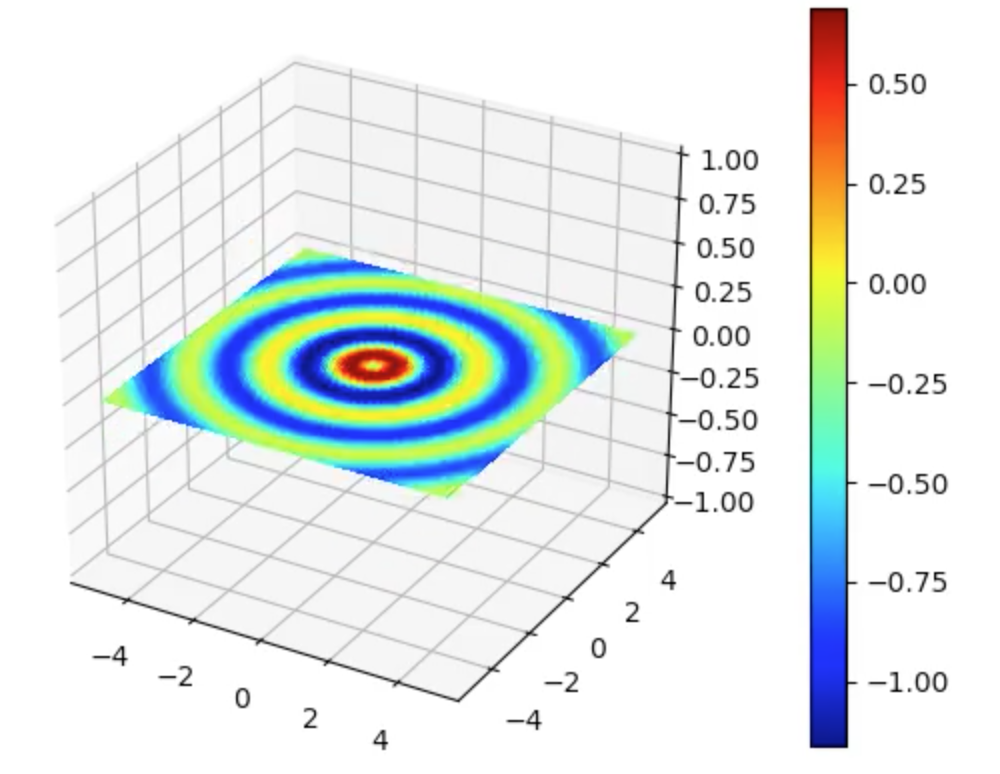
\includegraphics[width=\linewidth]{simulation/basich0.png}
        \caption{Wave motion at $h=0$}
    \end{subfigure}
    \begin{subfigure}{0.5\textwidth}
        \centering
        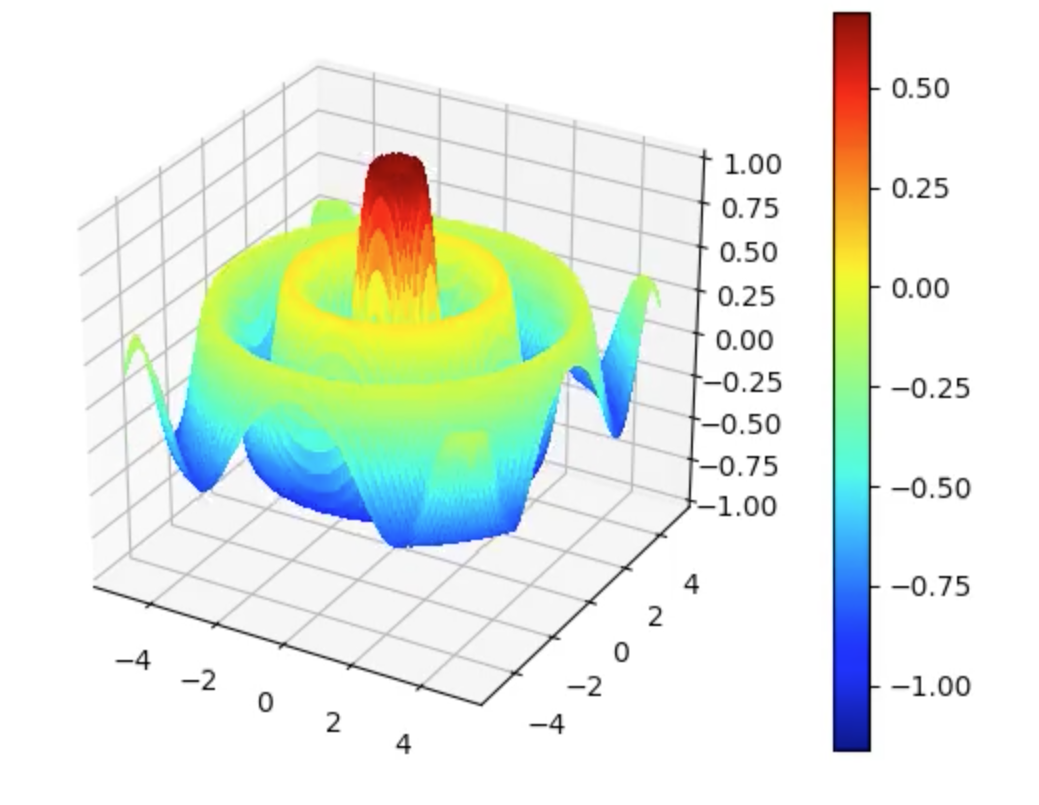
\includegraphics[width=\linewidth]{simulation/basichmax.png}
        \caption{Wave motion at $h=h_0$}
    \end{subfigure}
\caption{Simulation output generated with python and Matplotlib. (a) represents the initial state of the wavefield, while (b) represents the state of the wave-field when the "droplet" at the centre is at its maximum height}
\label{fig:basicAnimation}
\end{figure}


\subsection{Constructing a GUI in Java}
Initially, a Java simulation was developed, which aimed to construct a pixel grid which could be used to represent a wave-field. Objects representing a given data point and a "frame" of these data points were constructed, and populated with amplitudes using (\ref{equ:basicHeight}). These amplitudes were then displayed in 2D by assigning them to an opacity scale, with 100\% opacity representing the maximum possible height and 100\% transparency representing the minimum possible height. For a 40,000 pixel frame running over 10 seconds, this process took approximately 9 seconds, but the animation process after this ran in real time. Figure \ref{fig:javaBasicHeight} shows a still image of this GUI taken when the "droplet" was at a minimum height of $-h_0$. This animation was a success, but at higher resolutions, latency when drawing the pixels to the screen caused it to lag, suggesting a need to either run multiple drawing tasks in parallel, or to display the droplet motion in an alternative way.

\begin{figure}
    \centering
    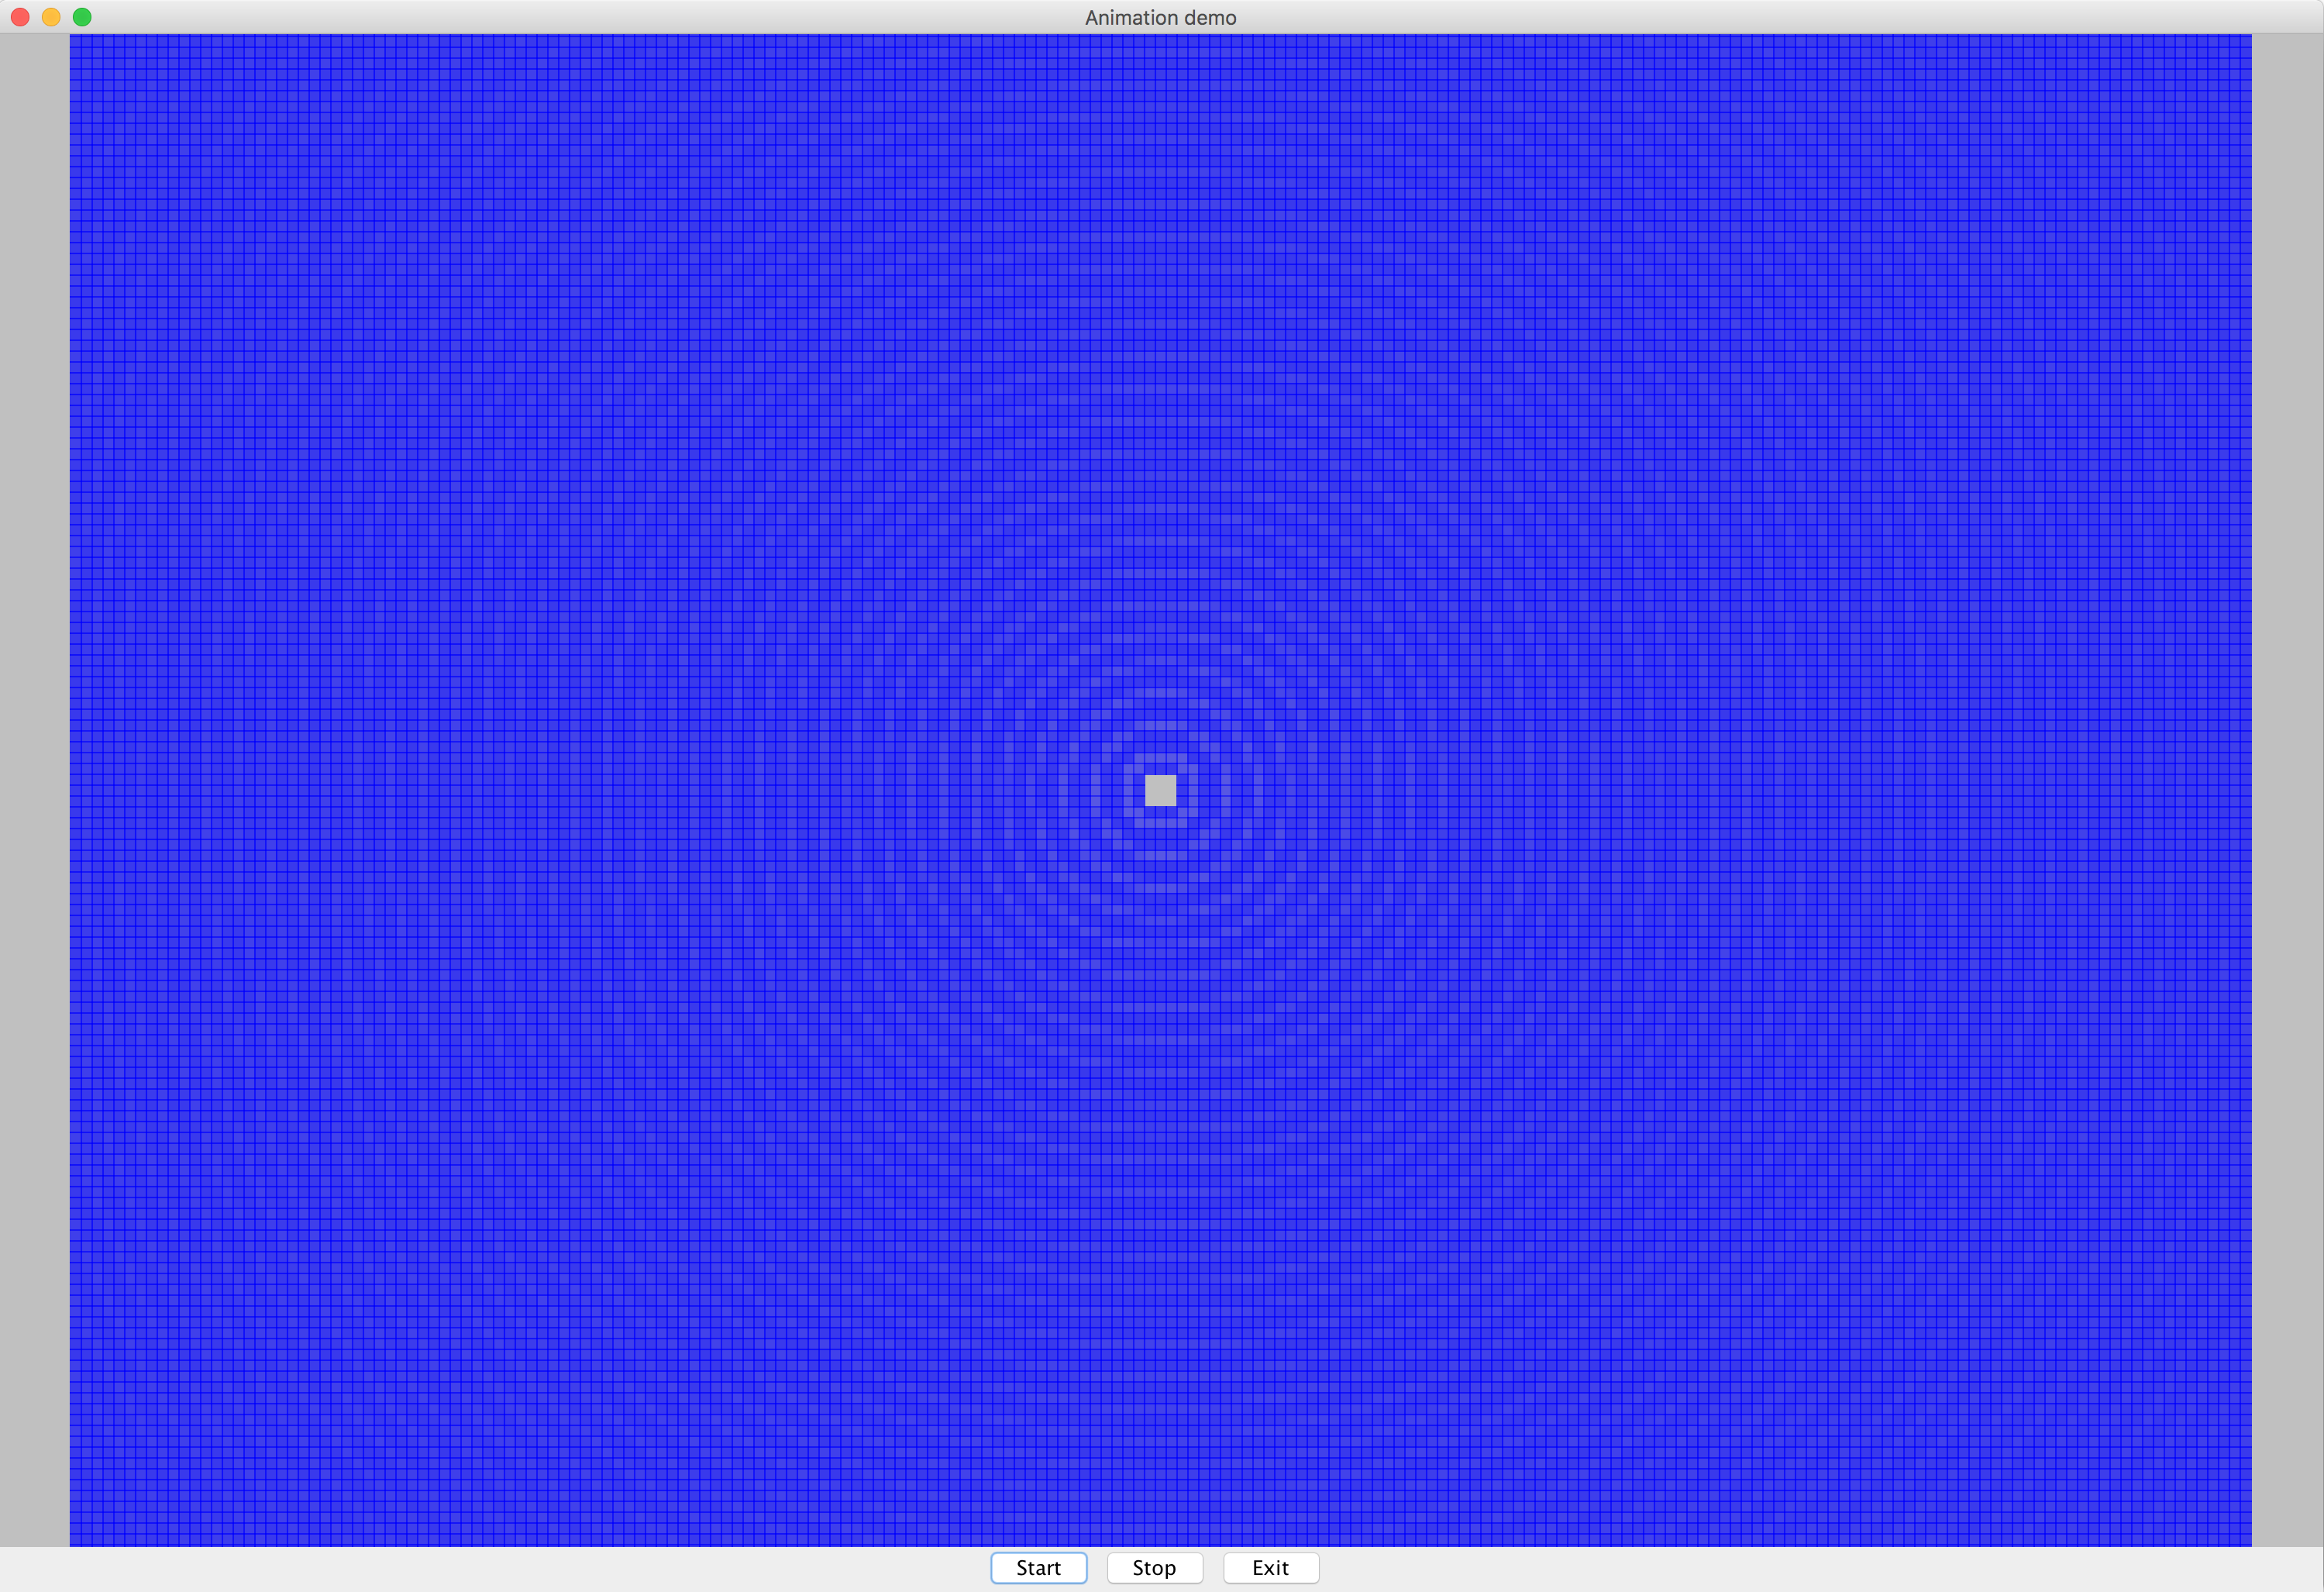
\includegraphics[width=\textwidth]{simulation/javaMaxHeight.png}
    \caption{A basic Java GUI, here showing the droplet at its minimum height of $-h_0$}
    \label{fig:javaBasicHeight}
\end{figure}

\subsection{Probabilistic prediction of position}
Having demonstrated the possibility of displaying wavefunctions in Java, displaying an object representing a droplet was the next task. Here, the assumption was that the wave (described by (\ref{equ:probWaveEqn})) represented a probability density function. Therefore, for a given (and ideally infinitesimal) pixel n of area dA, the probability $P_n$ of finding the particle at pixel $n$ was calculated from that function. The height ($z_n$) of each pixel within that section was calculated, with ${P_n}/{z_n}$ representing the probability of the particle being at that pixel. The sum of probabilities for this section, $Z=\sum_n{P_n}$, defined the normalisation value of the thread. A random number generator then generated a number R such that $0\leq R \leq 1$, which was multiplied by $Z$ to give a relative random number. The program then looped back over all the pixels in the section, and repeatedly subtracts $P_n$ from $RZ$ until $RZ<0$. The first pixel where this condition is satisfied is determined to be the location of the droplet. This process could then be multi-threaded to improve computational efficiency.

The application of this to our project was that once the droplet is found at a given pixel, the distance between that pixel and the next pixel representing the location of the droplet is used to calculate the velocity $v$ of the particle, assuming the droplet moves to the new pixel in the space of one period $T=1/f$. The wavefunction was updated with the new velocity, once a Lorentz transform was accounted for. This whole process is repeated to find the trajectory of the pixel.

\begin{figure}
\centering
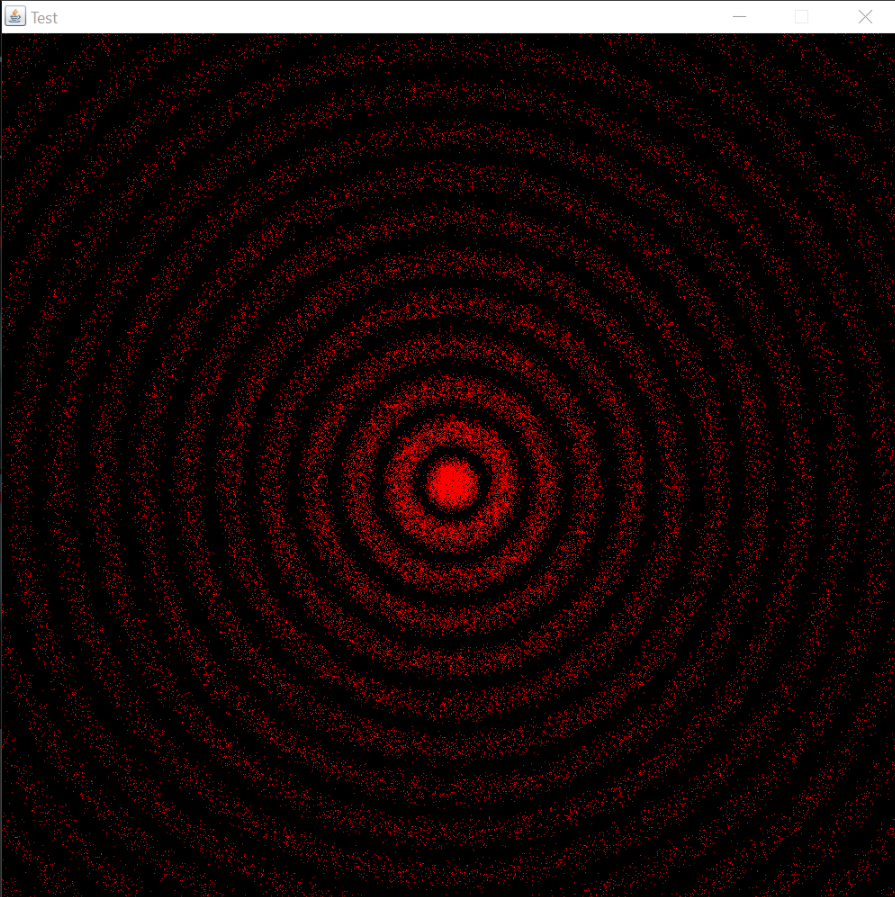
\includegraphics[width=\textwidth]{simulation/probabiltyPosition.png}
\caption{Results of the probabilistic prediction of the droplet position, where each dot represents the droplet being present at this point}
\label{fig:probabilisticPrediction}
\end{figure}

\begin{equation}
    h = -\cos(\omega t) J_0(\frac{\omega}{c} |\vec{r_f}-\vec{r_i}|)
    \label{equ:probWaveEqn}
\end{equation}

Although this process was successful, all it ended up proving was that a random position generator works. It does not accurately simulate the position of droplets created in our experiment. Therefore, we proceeded to calculate the equations of motion and the wavefunction of the droplet at each point.

\todo{Finalise writeup of MATLAB work}
\subsection{Rapid prototyping in MATLAB}
In parallel to this, MATLAB was chosen to test implementations of mathematical concepts found in our research, as it has a wide variety of built in libraries, such as for graphing software and advanced mathematical processes. Initially, equations of motion for the droplet were taken from \cite{oza2013trajectory}, where (\ref{equ:MATLABPilotWave}) defines the wave-field of the particle and (\ref{equ:MATLABWaveHeight}) defines the bath height over time. To implement these, a grid object was constructed and populated with x-y coordinates. A point in the middle of the grid was then selected as the starting position for a droplet, which was used as the centre of modelling for the first interaction.

\begin{equation}
m \vec{x}'' + D\vec{x}' + k\vec{x} = -mg\nabla h(\vec{x},t)
\label{equ:MATLABPilotWave})
\end{equation}

\begin{equation}
h(\mathbf{x},t) = \sum_{n=-\infty}^{\floor{t/T_F}} A \mathbf{J}_0(k_F |\mathbf{x}-\mathbf{x}_p(nT_F)|) e^{-(t-nT_F)/(T_F Me)}
\label{equ:MATLABWaveHeight}
\end{equation}

Once a centre had been chosen, the wave-field generated by the droplet at that point was calculated at time $t=0$. Assuming that the droplet bounces in phase with the forcing frequency, the droplet next interacts with the bath at time $t=T_F$, where $T_F = 2/\omega$, with $\omega$ representing the forcing frequency of oscillation. The evolution of the wave-field during this time period was calculated from the Bessel function $\mathbf{J}_0$, and so the droplet experiences a quasi-instantaneous acceleration proportional to the gradient of the wave-field at the droplet's position. A wave-field is generated at the droplet's new position following this acceleration. This process is repeated, with the $N$ most recent wave-fields added to the current wave-field, where $N$ represents the number of recent impacts used to calculate the wave-field. Each iteration of this process was represented with a frame in the animation, which contained a colour-coded $(x,y,z,t)$ point for the entire grid, as shown in Figure \ref{fig:MATLABMaths}.
\begin{figure}
\centering
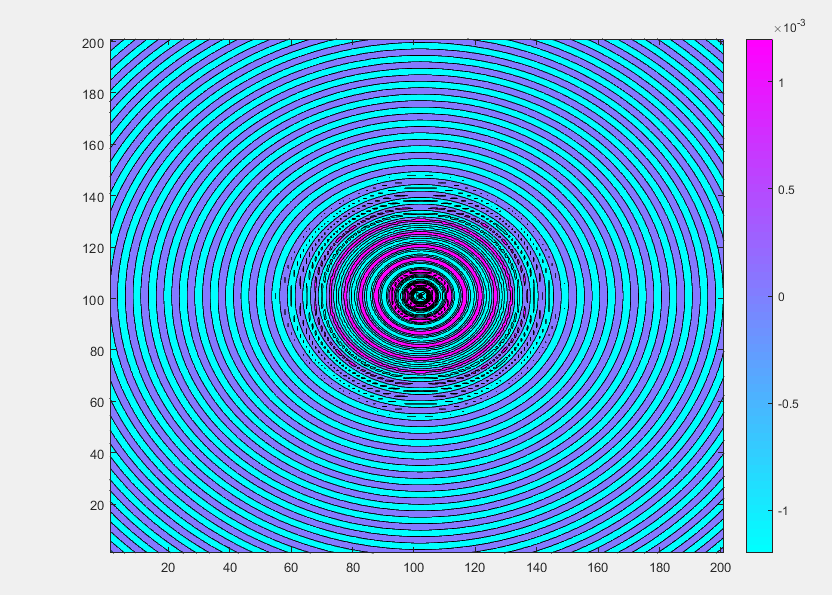
\includegraphics[width=\textwidth]{simulation/matlab.png}
\caption{The wave-field of a single droplet after multiple iterations, with a box size of 200x200 pixels and $N$=16. $N$ was chosen as the machine used was capable of 8 threads and each impact is calculated in parallel}
\label{fig:MATLABMaths}
\end{figure}

\subsection{Modelling assumptions and simulation mechanics}

The following assumptions were made during the simulation: 

\begin{enumerate}
\item The particle and surface waves produced are oscillating in phase with each other.
\item The particle and surface only interact within a small time frame $T_i$, after the particles' lowest point.
\item The average force exerted by the particle over $T_i$ is given by an effective wave force $F_b$. $F_b$ depends on material parameters and the mass of the particle, and tt has a maximum magnitude equal to the weight of the particle.
\item The effect of the Lorentz transform is negligible.
\item The impulse applied to the particle in the vertical direction perpendicular to the surface is assumed to be negligible and the particle continues oscillating vertically at the same frequency and amplitude. 
\item The particle experiences no damping force
\item The overall wave equation $h(\vec{r} , t)$ is dominated by the waves from the last $N$ bounces only. Waves formed longer than $N$ bounces ago are removed from the overall wave equation. This simplifies the computation of the infinite sum within the overall wave equation. In the Java simulation, by integrating multi-threading methods into our calculation, we were able to efficiently perform calculations with $N = 300$.
\end{enumerate}

Following these modelling assumptions, the parameters of the system were set as follows \cite{dotwave}:

\begin{itemize}
\item Particle mass, $m_p = 2.6\times10^{-7}$ kg
\item Driving Frequency $\omega= 80$ Hz
\item Period of particle, $T_f = \frac{2}{\omega}$ s
\item Gravitational acceleration, $g = -9.81$ m/s
\item Effective force, $F_b = 1.3174\times10^{-6}$ N
\item Wave number, $k = 1250$
\item Amplitude, A = $\frac{F_b}{m_pkg}$ m
\item N = 300
\end{itemize}


From the assumptions made above, it can be shown that the change in velocity of the particle in the direction parallel to the surface is given by:
\begin{equation} \Delta \vec{v} = \frac{T_i  F_b}{m_p} \times \frac{dh(\vec{x} , t)}{d\vec{x}}\end{equation}
Where $m_p$ is the mass of the particle and the last term is the vector gradient of the wave.


It was difficult to strike a balance between an acceptable data generation time and simulation accuracy. With simulation values used in the image above, each frame takes over 10 minutes to generate. The largest factor in the total processing time is the number $N$ of previous impacts stored. In the physical situation, the decay of each wave generated at an impact would be dependent only on the $Me$ parameter. \cite{couder11} In numerical simulation, only a limited number of recent impacts can be stored within the memory but ideally the value of $N$ should be chosen such that the contribution of an impact is nearly negligible when it is removed from memory. However, due to computational limitations, only the 16 most recent impacts were used in the calculation of the wave-field. This also precludes the simulation of multiple droplets, as each droplet would result in an additional $N$ impacts being stored.

The issues encountered in terms of processing speed could be partially addressed by porting the mathematical model developed into Java.  While it was expected that this would enable more efficient data generation, the realistic improvement in speed that could be offered would not be able to entirely negate these problems.
It was clear at this point that, regardless of potential optimisation, the goal of having a interactive simulation was not within the scope of the project. It was subsequently  decided to focus on using the previously developed Java graphics system with the aforementioned prototype  to create a number of pre-rendered videos.

\subsection{Integrating Java and MATLAB}

Due to calculation and graphical issues in  MATLAB and Java respectively, a possible solution was the execution of Java classes from a MATLAB script. This would allow the calculations to be carried out in Java, outputted to a csv or text file, and then read by the initial MATLAB script for demonstration. This was implemented using the command() function in MATLAB to navigate to the source folder, compile and then run the necessary classes. Due to time constraints, it was not possible to complete this. The main issue encountered was the use of external .jar files (to implement the Bessel function) not allowing the java files to compile. Various unsuccessful solutions were attempted,so it was decided to move on.



subsection{Java}

Importing the above model from MATLAB into Java was decided as the best course of action. The equations used and assumptions made were identical, but there was a slight difference in the manner which the gradient was calculated.

As opposed to using a built in function, in 1-D, the gradient at a point $x = x_0$ is given by:
\begin{equation} \frac{dy}{dx}\Bigr|_{x_0} = \lim_{x\to0} \frac{y(x+\delta x)-y(x-\delta x)}{2\delta x}\end{equation}

Using a Taylor expansion about $x_0$, it can be shown that for $\delta x\neq 0$:
\begin{equation} \frac{dy}{dx}\Bigr|_{x_0} = \frac{y(x+\delta x) - y(x-\delta x)}{2\delta x} - O(\delta x)\end{equation}
Where $O(\delta x)$ is the residual given by:
\begin{equation}O(\delta x) = \sum_{n=2}^{\infty} \left( \frac{y^{(n)}(x_0)}{n!\times (2\delta x)} \left[ \left( x+\delta x -x_0 \right)^n - \left(x-\delta x -x_0 \right)^n \right] \right)\end{equation}

The 2-D vector gradient of $h(\vec{r} , t)$ was determined by first finding the 1-D gradient in the x-direction by using $\delta \vec{r} = (\delta x,0)$, followed by that in the y-direction by using $\delta \vec{r} = (0,\delta y)$. The 1-D gradients in each direction corresponds to the component of the 2-D vector gradient in their respective directions. 

In our computational model, $|\delta \vec{r}| = 1\times 10^{-18}$ was used. The resolution of the Bessel functions used prevented the use of any value smaller than this. Attempts using $|\delta \vec{r}| = 1\times 10^{-19}$ resulted in gradients calculated to either have magnitude 0 or magnitude $\approx 30$, which does not match the shape of the first order Bessel function.

The wave velocity was calculated to be $\approx 0.201$. The perturbation velocity was on the order of 0.001, corresponding to $\gamma = 1.00001$. For simplicity of simulation, the Lorentz effects were assumed to be negligible, and left out of calculation.

The simulation was produced by creating .png files in Java, then stitching them into a video using VirtualDub, which could then be presented to others.

\subsection{Simulation in the high- and low-memory regimes}

The goal of the first simulation was to show that walking occurs as a result of the high memory regime. To test this, two simulations were run, one at Me = 150 and one at Me = 15. In both simulations, N = 300 was used. The particle was allowed to first bounce on the spot to build up 300 waves in the overall wave equation, corresponding to t = 7.5s. The particle was then perturbed by spontaneously changing its velocity to $\vec{v} = (0.0005,0)$. The results of the high and the low memory regime simulations are shown in Figure \ref{fig:memory}. 

\begin{figure}
	\centering
	\begin{subfigure}{\textwidth}
		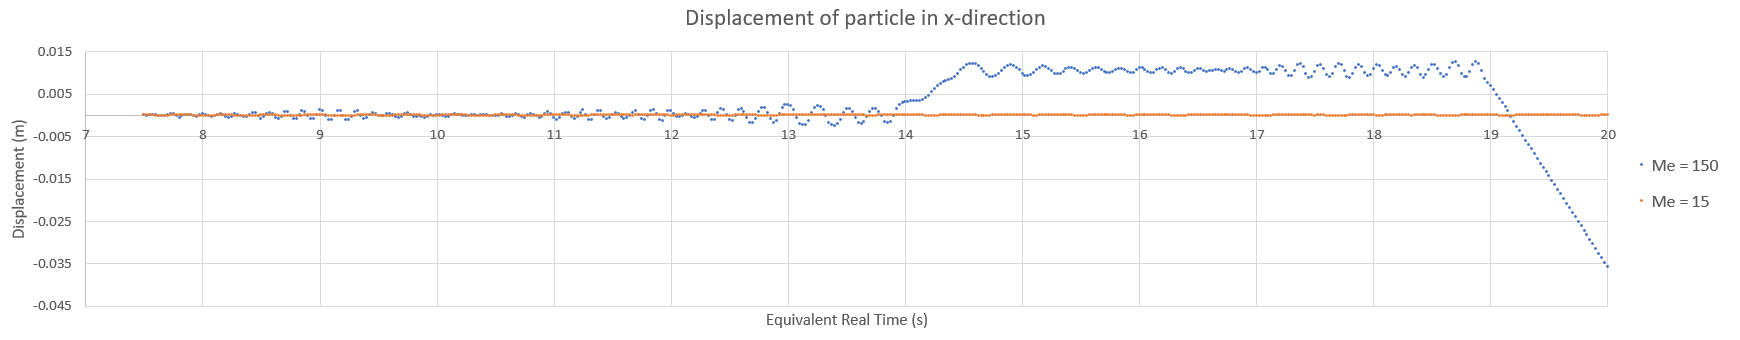
\includegraphics[width=\textwidth]{simulation/highmemory/displacement.png}
		\caption{Graph of displacement in the x-direction over time. $Me=150$ represents the high memory regime, whereas $Me=15$ represents the low memory regime}
		\label{fig:mem:displacement}
	\end{subfigure}
	
	\begin{subfigure}{\textwidth}
		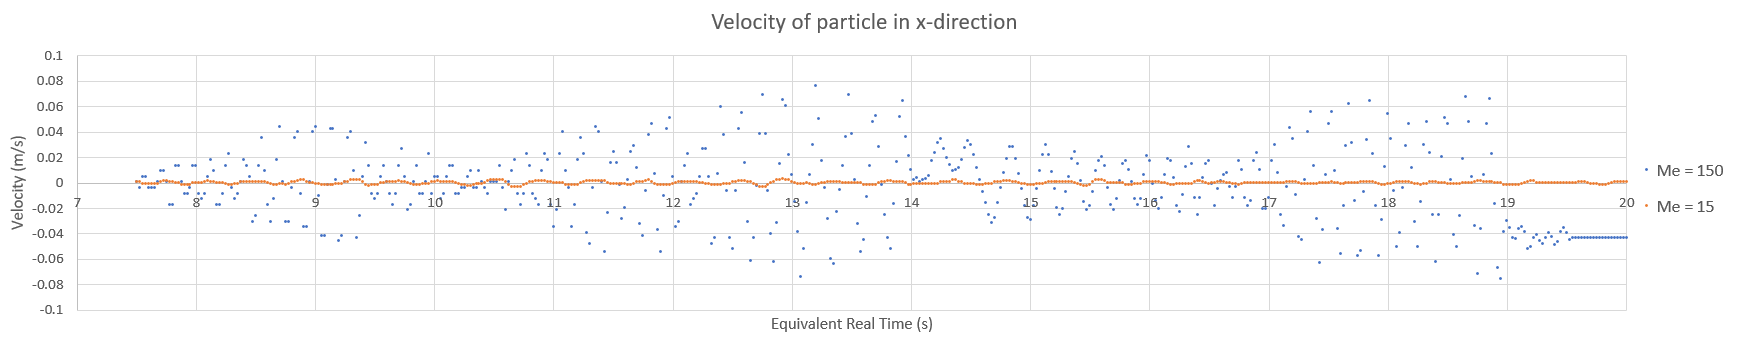
\includegraphics[width=\textwidth]{simulation/highmemory/velocity.png}
		\caption{In the high-memory regime, the particle velocity fluctuates chaotically before entering a stable state $\approx 11$s after perturbation. In the low-memory regime, the particle has negligible velocity}
		\label{fig:mem:velocity}.
	\end{subfigure}
	
	\begin{subfigure}{0.475\textwidth}
		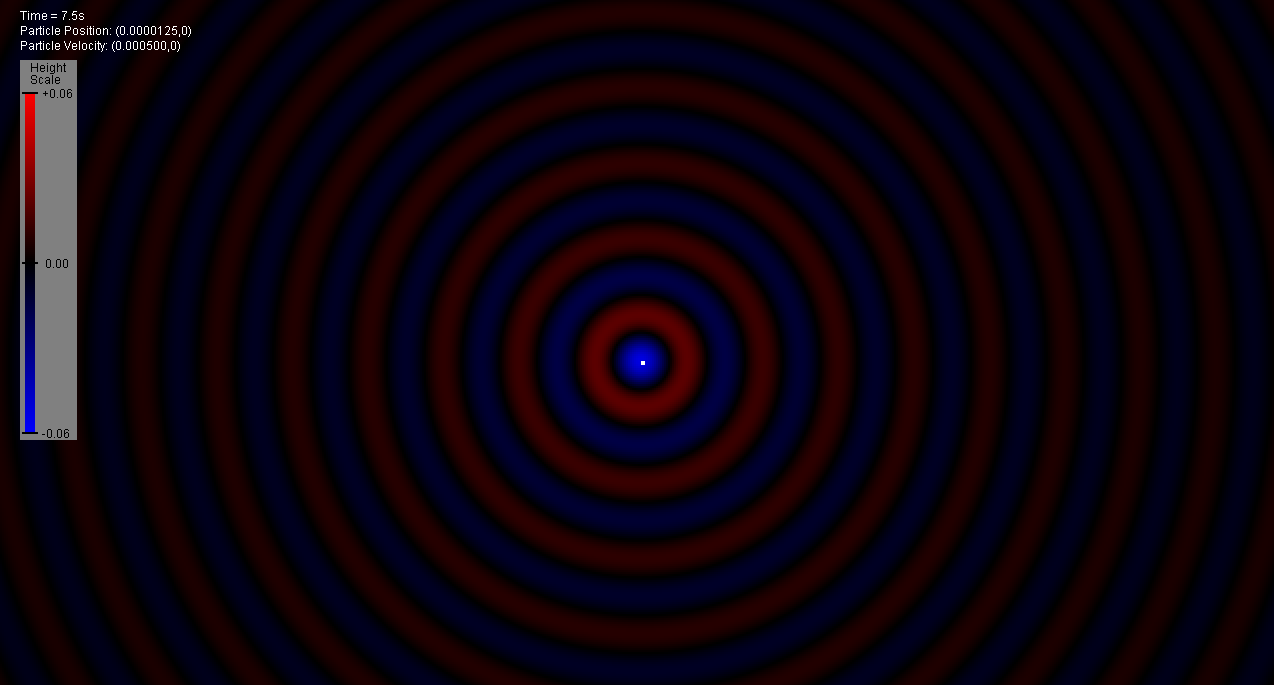
\includegraphics[width=\textwidth]{simulation/highmemory/wavefield75.png}
		\caption{The overall surface wave after $7.5$s; the wave-field has a similar shape to a 2-D harmonic potential well}
		\label{fig:mem:wavefield75}
	\end{subfigure}
	\hfill
	\begin{subfigure}{0.475\textwidth}
		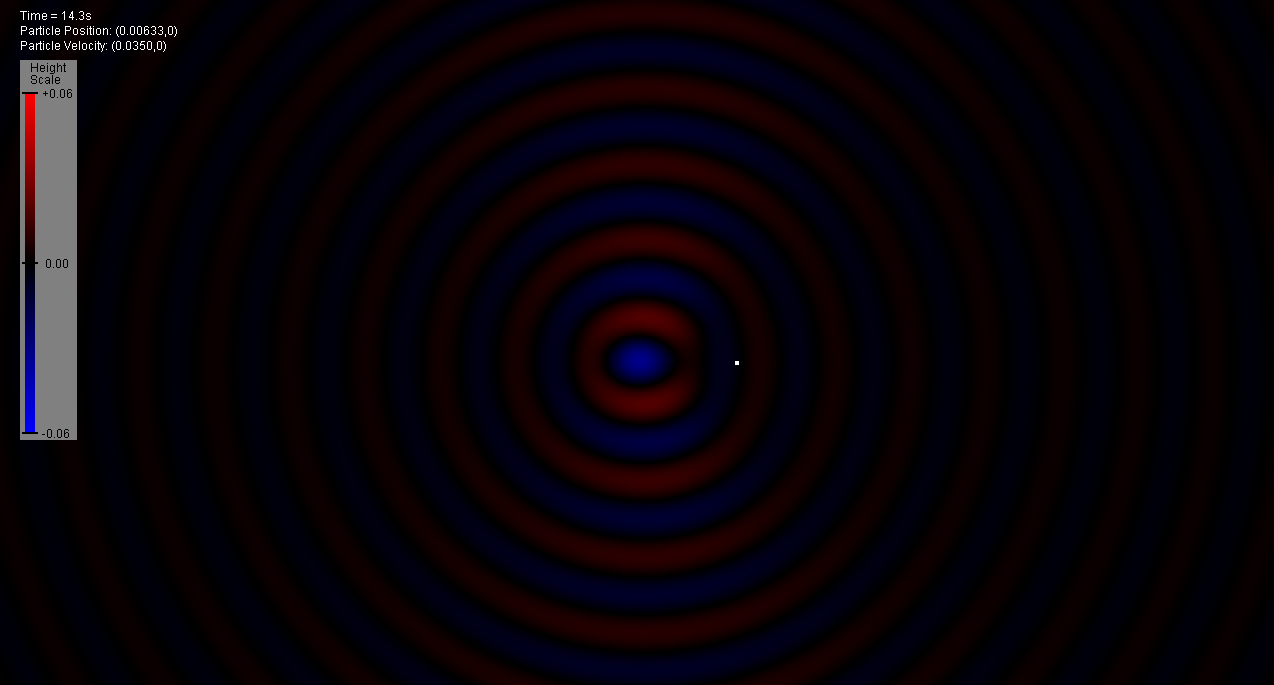
\includegraphics[width=\textwidth]{simulation/highmemory/wavefield145.png}
		\caption{The wave-field at $14.5$s, just prior to the particle breaking through the potential barrier and travelling}
		\label{fig:mem:wavefield145}
	\end{subfigure}
	
	\begin{subfigure}{0.475\textwidth}
		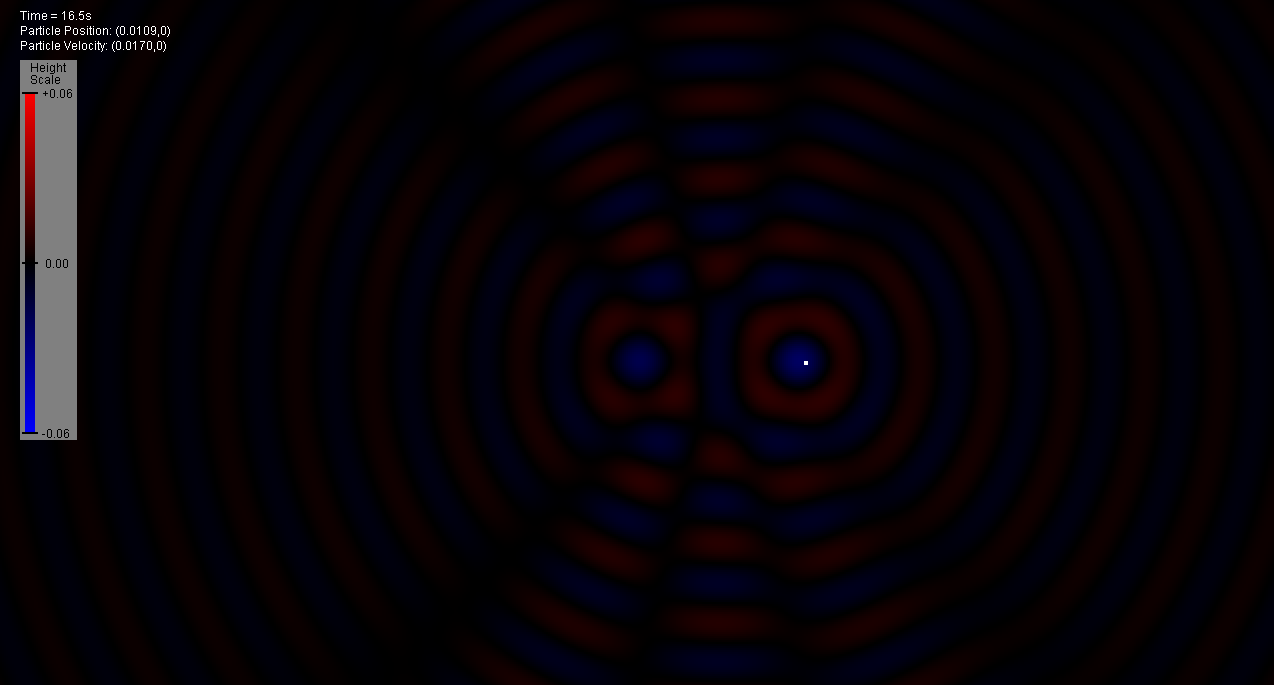
\includegraphics[width=\textwidth]{simulation/highmemory/wavefield165.png}
		\caption{Following multiple interactions with wave peaks, the particle decelerates and reforms a potential well}
		\label{fig:mem:wavefield165}
	\end{subfigure}
	\hfill
	\begin{subfigure}{0.475\textwidth}
		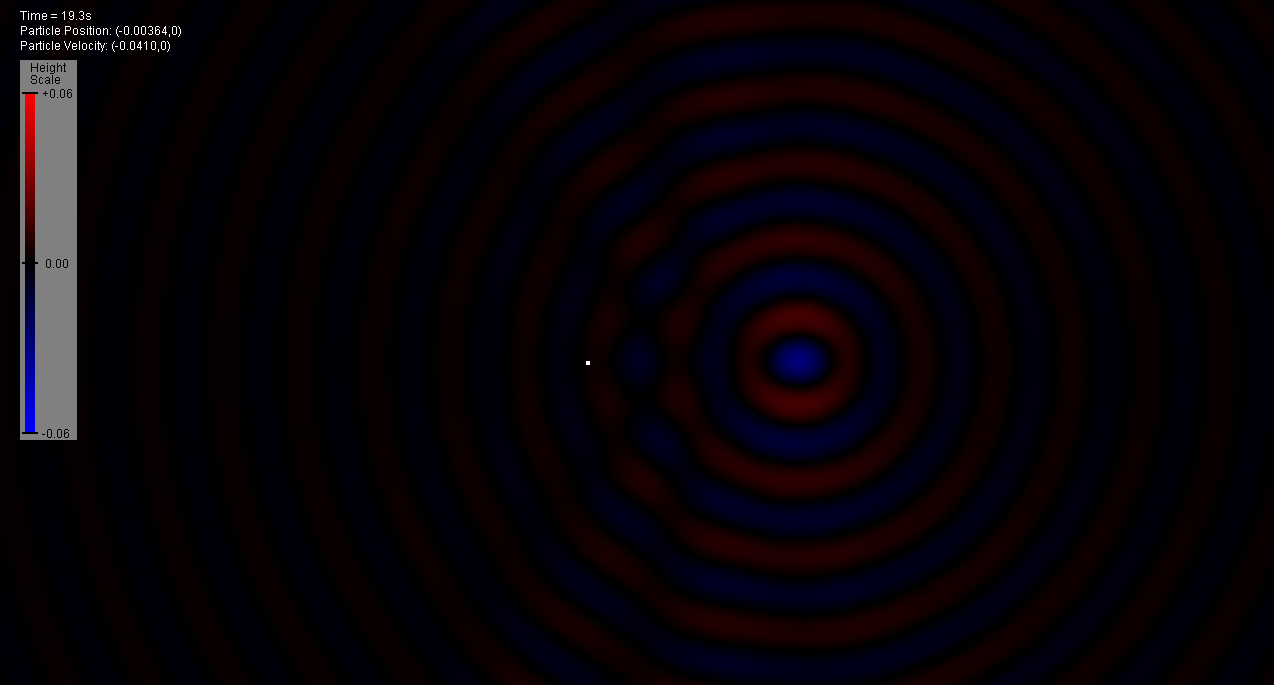
\includegraphics[width=\textwidth]{simulation/highmemory/wavefield195.png}
		\caption{The stable wave-field at $19.5$s, now displaced by $0.01m$.}
		\label{fig:mem:wavefield195}.
	\end{subfigure}
\caption{Results of the simulation in the high- and low-memory regime at different time periods}
\label{fig:memory}
\end{figure}

We see from Figure \ref{fig:mem:velocity} that the particle velocity is chaotic. This causes the particle to oscillate around two centres of displacement, initially the start position, and later about the point $(0.01,0)$. We also observe in Figure \ref{fig:mem:wavefield75} that, prior to perturbation, the wave-field is similar in shape to a 2-D harmonic potential well, of width $\lambda/2$, and centred about the initial position of the particle. Upon perturbation, the particle oscillates, as expected for such a system. However, with each impact at positions away from the start position, new waveforms are added to the overall wavefunction at these points. The waves formed at this point superpose over the 2-D harmonic potential well, flattening it along the x-axis. After approximately 7s, the peaks at $\lambda/2$ away from the start position along the x-axis were low enough that the particle could leave the well as shown in Figure \ref{fig:mem:wavefield145}.

The overall surface wave at 7.5s is shown in Figure \ref{fig:mem:wavefield75}. The wavefield is observed to be similar in shape to the 2-D harmonic potential well within a half wavelength about the particles' start position. At this point, the particle is perturbed. As expected for a particle oscillating in a 2-D harmonic potential, the particle enters oscillatory motion. However, with each impact at positions away from the start position, new waveforms are added to the overall wavefunction at these points. The wave forms at this point superpose over the 2-D harmonic potential well flattening it along the x-axis. After approximately 7s, the peaks at half wavelength away from the start position along the x-axis were low enough that the particle could traverse it and leave the well about the start position. The overall surface wave at this point is shown in Figure \ref{fig:mem:wavefield145}. As the particle carries on in its trajectory away from the start position, it interacts with other smaller peaks, causing it to slow down. As the particle slows down, the most recently formed waves are centered closer and closer together, eventually reforming yet another potential well about the point (0.01,0). The overall surface wave at this point is shown in Figure \ref{fig:mem:wavefield165}. The particle then starts oscillating about this point for approximately 4s before the same mechanisms that allowed it to break through the first potential well occurs, and the particle leaves the new formed well. Following this the particle enters a steady state and continues travelling with a stable velocity of (-0.043,0) $ms^{-1}$. The particle has thus started ``walking".

The high memory regime simulation was repeated for perturbation velocity with magnitude between 0.0001 $ms^{-1}$ and 0.0020 $ms^{-1}$ at intervals of 0.0001 $ms^{-1}$, to ensure that the above result of achieving walking was not due to specifically selected variables. In all cases the particle entered a steady ``walking" state with velocities ranging form magnitude 0.00859 to 0.102. The final steady state velocities of each particle and their corresponding perturbation velocity can found in \ref{fig:pertVfinal}. No observable trend was found relating the steady ``walking" state velocity and the perturbation velocity.
\begin{figure}
    \centering
    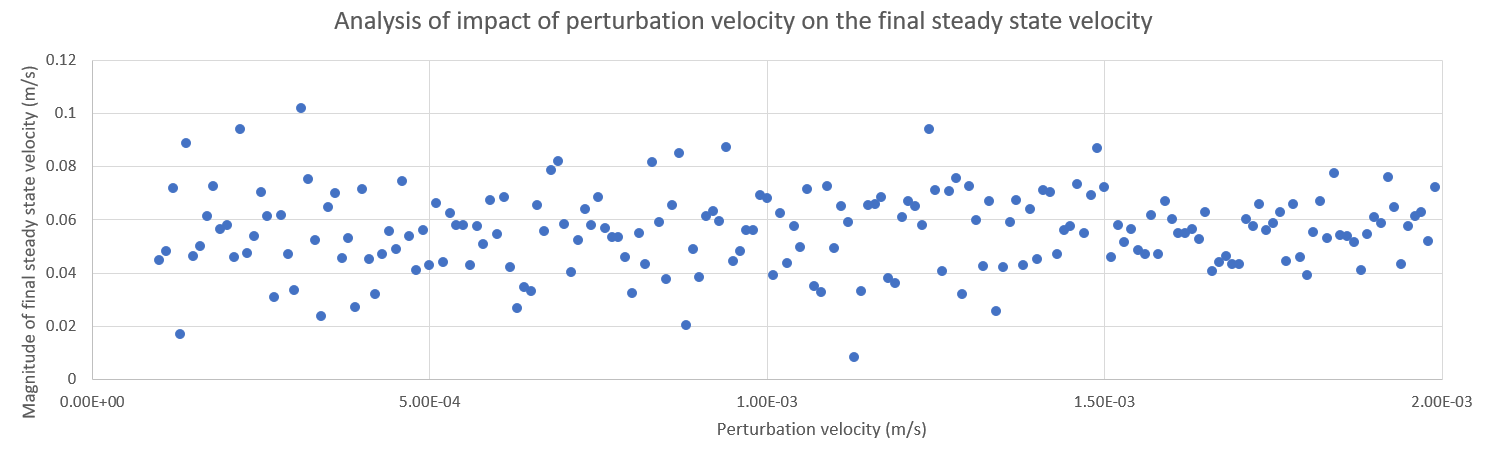
\includegraphics[width=\textwidth]{simulation/figpert.png}
    \caption{Results of the simulations in the high memory regime at velocities ranging from 0.0001 $ms^{-1}$ and 0.002 $ms^{-1}$}
    \label{fig:pertVfinal}
\end{figure}

The above results strongly suggest that a particle entering the walking state depends on $Me$. Simulations were next conducted for $Me$ between 15 and 150 at intervals of 0.1. Perturbation velocity was kept constant at (0.0005,0) $ms^{-1}$ in all simulations. The following conditions were set to determined if the particle has entered a walking state:

\begin{enumerate}
    \item $\Delta\vec{v} = 0$ for the past 20 time steps.
    \item The particle is at least 1 wavelength away from where it was initiated.
\end{enumerate}

If the particle in a simulation was detected to be in a walking state, the simulation would output the walking state velocity and the time at which "walking" was achieved. Each simulation was allowed to run for 10,000 time steps, corresponding to 250s in real time. Any particle yet to achieve walking within this time frame was assumed to not be capable of entering the walking state. Visualisations of this data are shown as graphs in Figure \ref{fig:varmem}. 

As shown in Figure \ref{fig:varmem:walkingstate}, there is no clear threshold $Me$ beyond which the particle will enter a walking state. From the plot it is observed that walking will not occur for $Me < 50$ but will occur for $Me > 80$. The region in between, given by $50\leq Me\leq80$, however, appears to be a grey area where whether a given Me leads to a walking state seems to follow some distribution. To determine the shape of this distribution a moving average of the previous 20 and next 20 points was plotted against $Me$. By observation, the plot here appears to be in the shape of a sigmoid curve. Using Origin Pro 2017s' non-linear curve fit function, the plot in was fitted to a Boltzmann sigmoid function with the top and bottom value fixed at 1 and 0 respectively. The Boltzmann sigmoid is given by \ref{equ:BoltzmanSigmoid}.

\begin{equation}
y = (bottom) - \frac{(top)-(bottom)}{1+exp \frac{\left(x_0 - x \right)}{dx}}
\label{equ:BoltzmanSigmoid}
\end{equation}

Here $x_0$ is the 50\% threshold found to be $64.54\pm0.04$.

The fit was found to have a R-squared value of 0.9974 and a reduced chi squared value of $5.33 \times 10^{-4}$ suggesting a decent fit. The plot of the residual of the fit against $Me$, as shown in Figure \ref{fig:varmem:residualplot}, interestingly seems to be in the form of a wave packet. 

Figure \ref{fig:varmem:timewalking} shows the relation between time taken to enter the walking state and $Me$. It is observed that the time taken has a wider spread for lower Me, with a minimum that remains constant as Me increases. The minimum has a value of approximately $3\pm2$. This corresponds to the time required to flatten the sides of the wave as described previously, thus allowing the particle to pass through it and leave the potential well around it.

The plot of the x-component of the walking velocity against $Me$ is shown in Figure \ref{fig:varmem:walkingvel}. Since the particle was perturbed in the x-direction only, the y-component in all cases is 0. It is observed that approximately half of the simulations produced a walking velocity in the positive x-direction (the direction of perturbation), while the remaining half in the negative x-direction. 



\begin{figure}
	\centering
	\begin{subfigure}{\textwidth}
		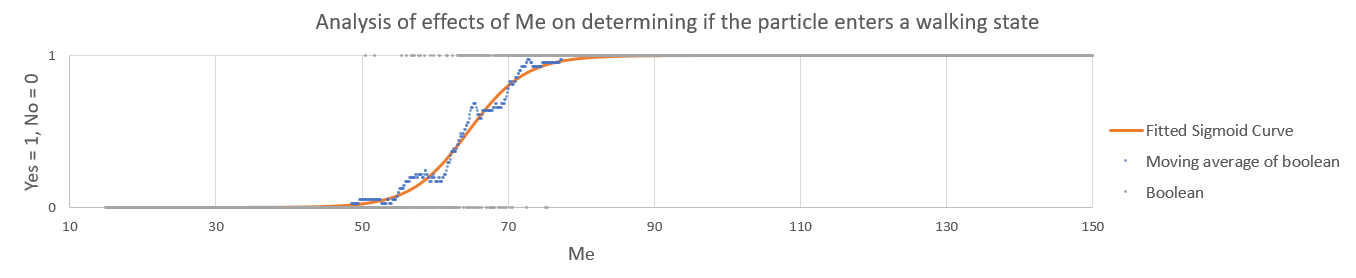
\includegraphics[width=\textwidth]{simulation/varmemory/walkingstate.png}
		\caption{Binary plot showing whether a particle was found to have entered a walking state within 10,000 time steps with 1 corresponding to yes and 0 to no against $Me$. The moving average is plotted and fitted to a sigmoid curve}
		\label{fig:varmem:walkingstate}
	\end{subfigure}
	 \begin{subfigure}{\textwidth}
		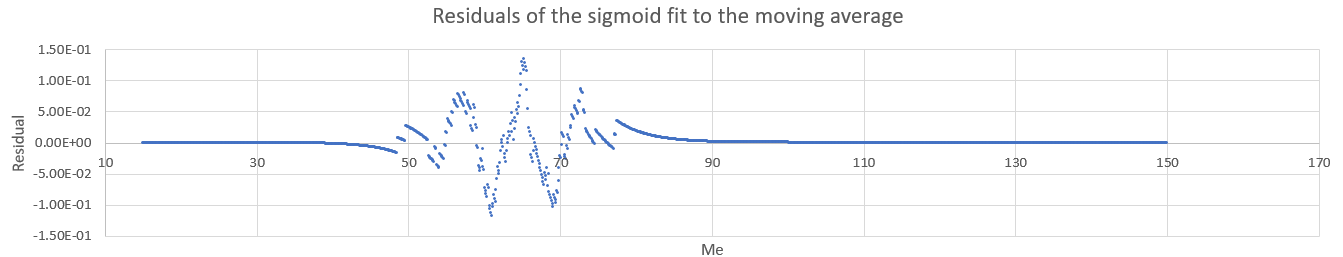
\includegraphics[width=\textwidth]{simulation/varmemory/residuals.png}
		\caption{Residual plot of the sigmoid fit of \ref{fig:varmem:walkingstate}}
		\label{fig:varmem:residualplot}
	\end{subfigure}
	\begin{subfigure}{\textwidth}
		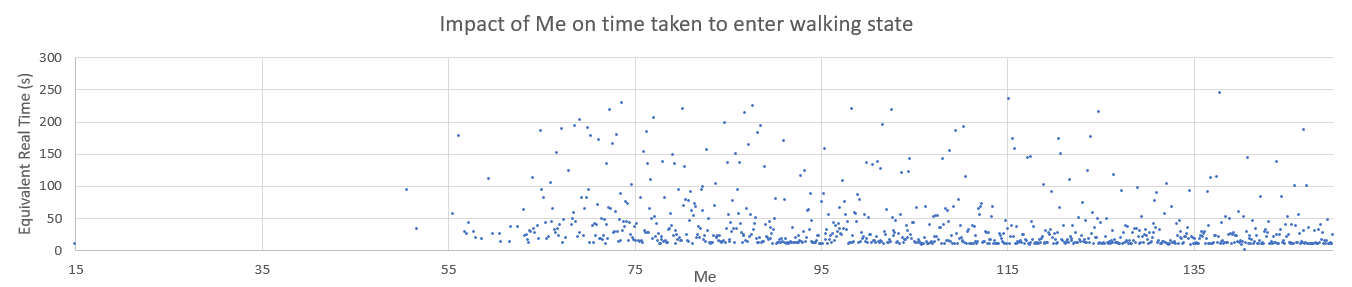
\includegraphics[width=\textwidth]{simulation/varmemory/meWalkingState.png}
		\caption{Plot of time taken for the particle to enter walking state against $Me$ used in the simulation}
		\label{fig:varmem:timewalking}
	\end{subfigure}
	
	\begin{subfigure}{\textwidth}
		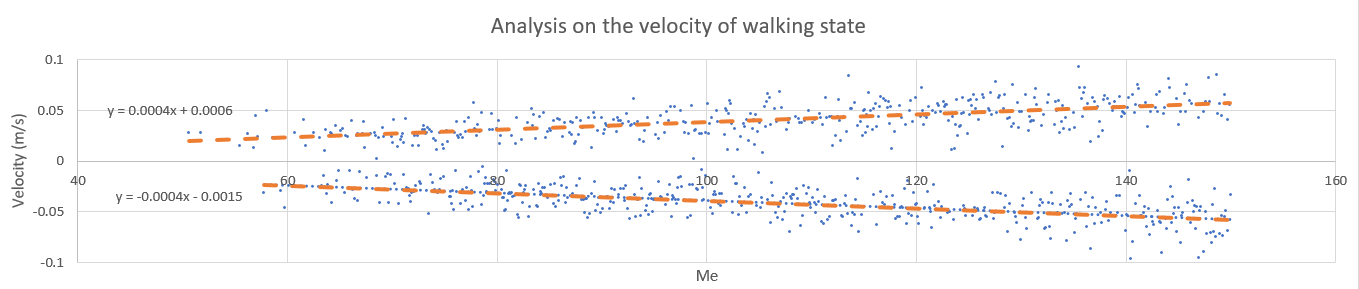
\includegraphics[width=\textwidth]{simulation/varmemory/velocityWalkingState.png}
		\caption{Plot of walking velocity of the particle against $Me$ used in the simulation}
		\label{fig:varmem:walkingvel}
	\end{subfigure}
\caption{Analysis of the probability of a particle entering the walking state at different values of $Me$}
\label{fig:varmem}
\end{figure}

\subsection{Preliminary tests on predicted phenomena}
The theoretical models used in our simulations also made other predictions as to the behaviour expected. To further provide supporting evidence for the validity of our  assumptions, we attempted to demonstrate some of these predictions. Due to time constraints, we only managed to run preliminary tests demonstrating oscillating droplets and wall repulsion.

\subsubsection{Oscillating droplets}

As predicted, \cite{brady2014bouncing} bouncing droplets experience an attractive force when they are bouncing in phase. Experimental evidence provided by the same team suggests that this force follows an inverse square relation similar to gravity and electromagnetism. A preliminary test was conducted by performing a simulation that initiated two droplets, separated along the x-axis by 0.004m. The droplets were initiated with velocities in the y-direction with magnitude 0.0003 $ms^{-1}$ in opposite directions. This resulted in the droplets having an angular orbital momentum between themselves.

In the simulation performed, it was observed that the droplets initially entered some form of orbital motion, as expected from an attractive inverse square force. However, orbital motion was only maintained for an equivalent real time of approximately 6s before the system destabilises. The droplets were then observed to enter walking states in opposite directions. Due to time constraints, further detailed analysis on the motion of the droplets were not performed. 

\subsubsection{Wall repulsion}

Wall repulsion was simulated by initiating a droplet displaced along the positive x-direction. A wall was positioned along the y-axis. By assuming the wall is completely reflective, an incoming wave should reflect off the wall out of phase, and in the direction given by the law of reflection. To simulate this, inspiration was taken from the method of mirror charges in electrostatics. Each time a waveform was added to the overall wave-function, a “mirror” waveform was also created. The “mirror” waveform added was out of phase with the droplet, and initiated at the position given by the reflection of the droplet in the y-axis.

The simulation demonstrated that the droplet accelerates away from the wall, as expected. Due to time constraints, no detailed analysis was performed on the motion of the particle so the trajectory of repulsion was not quantified. The effects of changing variables was also not explored.


\subsection{Conclusion}

The original aims of the simulation were to construct an interactive software package that could simulate and visualise the motion of droplets bouncing on a liquid surface. These aims were partially met: a non-interactive simulation was developed, whereby images from the software output could later be reconstructed into a video. However, due to computational limitations it was not possible to run this process in real time. This posed a significant barrier to the use of the simulation as a real-time educational aid, although the videos were still useful to illustrate the concepts to students in a classroom.

As work continued with the simulation, and the team developed a more detailed understanding of the theory behind droplet motion, additional goals were added to the project. This included determining the effect of changing simulation parameters such as the memory coefficient $Me$, and allowing the end-user to vary those without needing to understand the source code. Again, these were partially met: detailed analysis of the effect of $Me$ has been offered, an insight which would not be possible within the physical system. However, simulation parameters are still hard-coded, although this could change with relative ease in the future.

While a more quantitative analysis of boundary conditions and multiple droplets would have been desirable, the preliminary results obtained agreed with qualitative predictions. This suggests the simulation's behaviour is consistent with theory, but without quantitative comparisons, the accuracy of this could not be verified. This meant that the subsidiary goal of representing quantum effects, such as double-slit diffraction, was not met. To provide a more accurate model, several other factors that were assumed negligible could be accounted for, such as adding a parameter to represent the inelasticity of collisions between the droplet and the surface.
\spacing{1.2}

\clearpage
\section{Education and outreach efforts}
Having developed a portable prototype of the apparatus, investigations into its use as an educational tool were started. The aims of this part of the project were to identify the ability range of students who could benefit from such outreach, to develop and implement an outreach lesson, and assess its effectiveness in engaging students in undergraduate physics.

Considering the relatively high level of understanding of quantum physics required to grasp both the theory behind our experiment and its implications, sixth-form students were selected as the primary target group. To that end, teachers at schools project members had attended were contacted, and a school in Chesham selected for an outreach lesson. A lesson plan (Section \ref{lessonplan})) was developed, with significant feedback from Dr. Mark Fuller, outreach officer for the department. This, alongside a Powerpoint (Appendix \ref{app:powerpoint}), was delivered on the 7th March.

Evaluation of the lesson was conducted through a paper survey, overleaf, and through feedback from the class teacher. Students used a four point rate their agreement with various statements corresponding to our outreach aims. Each statement was then assigned an "agreement score", defined as $\frac{\sum{x}}{4N}$, where x is the score given to each statement and N is the number of students in the class. The results of this are shown in Figure \ref{fig:evaluationchart}.

\begin{figure}[h]
\centering
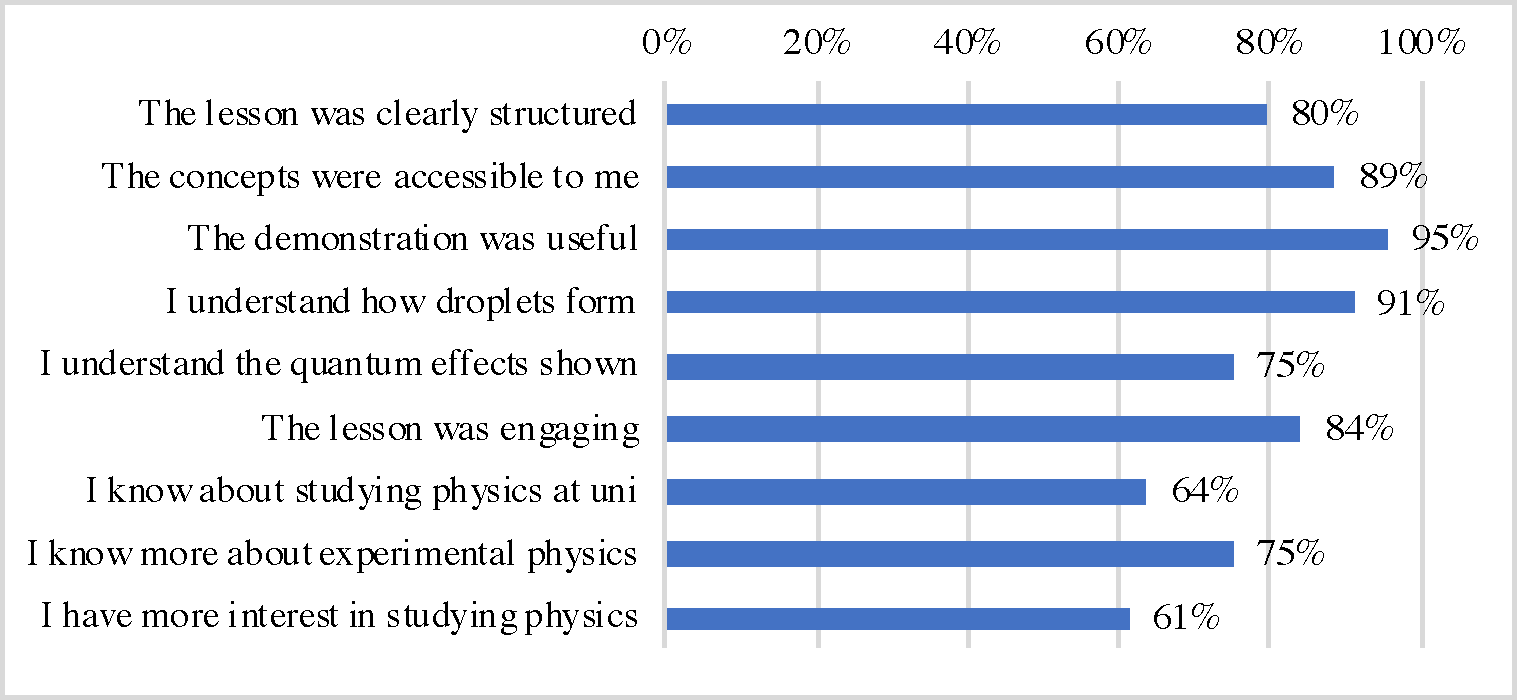
\includegraphics[width=\textwidth]{education/evaluationchart.pdf}
\caption{Percentage agreement with evaluation statements. Note that the final statement included a "not applicable" option, so has a smaller sample size.}
\label{fig:evaluationchart}
\end{figure}

This evaluation showed that students generally found the lesson enjoyable and engaging, and valued the use of the prototype as a demonstration aid. Understanding of the quantum effects shown by our experiment was less robust, although this could be due to the year 12 students being unfamiliar with such topics beforehand, as they don't study quantum physics in detail until year 13. Most lacking from this intervention was an understanding of the experience of studying physics at university. It would be relatively easy to devote more time to this in future sessions, depending on the precise aims of the workshop, which should provide sufficient improvement.

\clearpage

\subsection{Lesson Plan} \label{lessonplan}

\noindent Date: 7/3/18

\noindent Lesson: Physics

\noindent Year: 12/13

\noindent Levels: Any

\noindent Tutor: Group 13

\noindent Topic: Quantum mechanical effects using bouncing droplets


\noindent Learning objective and outcomes:
\begin{enumerate}
\item How droplets can bounce on a vibrating surface
\item What quantum mechanics is, and what effects we can observe some of these things from the apparatus
\item Have an insight into undergraduate physics and some of the hands on work it can entail
\end{enumerate}

\noindent \textbf{Introduction} (5 mins): Introduce ourselves and the reasons we're there for. 

\noindent \textbf{Starter} (10 mins): Start discussion into what quantum physics is. To facilitate audience participation, ask students to discuss amongst themselves for 3 minutes and propose ideas. Then ask for these ideas, and add/correct responses as required

\noindent \textbf{Mini-lecture} (10 mins): How do droplets form? (Diagram on board) Explain that (but not how) these droplets demonstrate QM behaviour. Starting from basic diagrams and maybe a recording of bouncing droplet motion, explain how droplets bounce. Then explain that these droplets replicate quantum behaviour. Attempt to limit the scope of this behaviour by mentioning specific effects. Don't explain how this link occurs yet.

\noindent \textbf{Demonstration} (10 mins): Explain apparatus and highlight important components. Execute a run through of the apparatus (need to find a way to get a live feed to projector). Specifically demonstrate bouncing droplets, walking droplets and multiple droplet motion. Take time to allow for students to run through experiment themselves, e.g. by making droplets and playing with the frequencies/bass. As there is only one apparatus, take suggestions from students. 

\noindent \textbf{Discussion} (10 mins): Discuss in groups how these droplets display behaviour. Ask students to also note down any interesting behaviours they observe. May have to use lab based recordings/ simulation for double slit diffraction or other interesting effects we want to mention

\noindent \textbf{Plenary} (10 mins): Assert that droplets demonstrate XYZ behaviour, make limitations clear. Wrap up by emphasising learning objectives, link to Veritasium for more details. It would be quite useful to part on an entertaining note. See if music/ colourful lights can make the apparatus do something more exciting. 

\noindent \textbf{End of session} (10 mins): 10' Q&A on Physics at Uni, completion of end of session assessments. 



\noindent \textbf{Key words}: Pilot wave theory, guiding wave equation, wave particle duality, Destructive and constructive interference

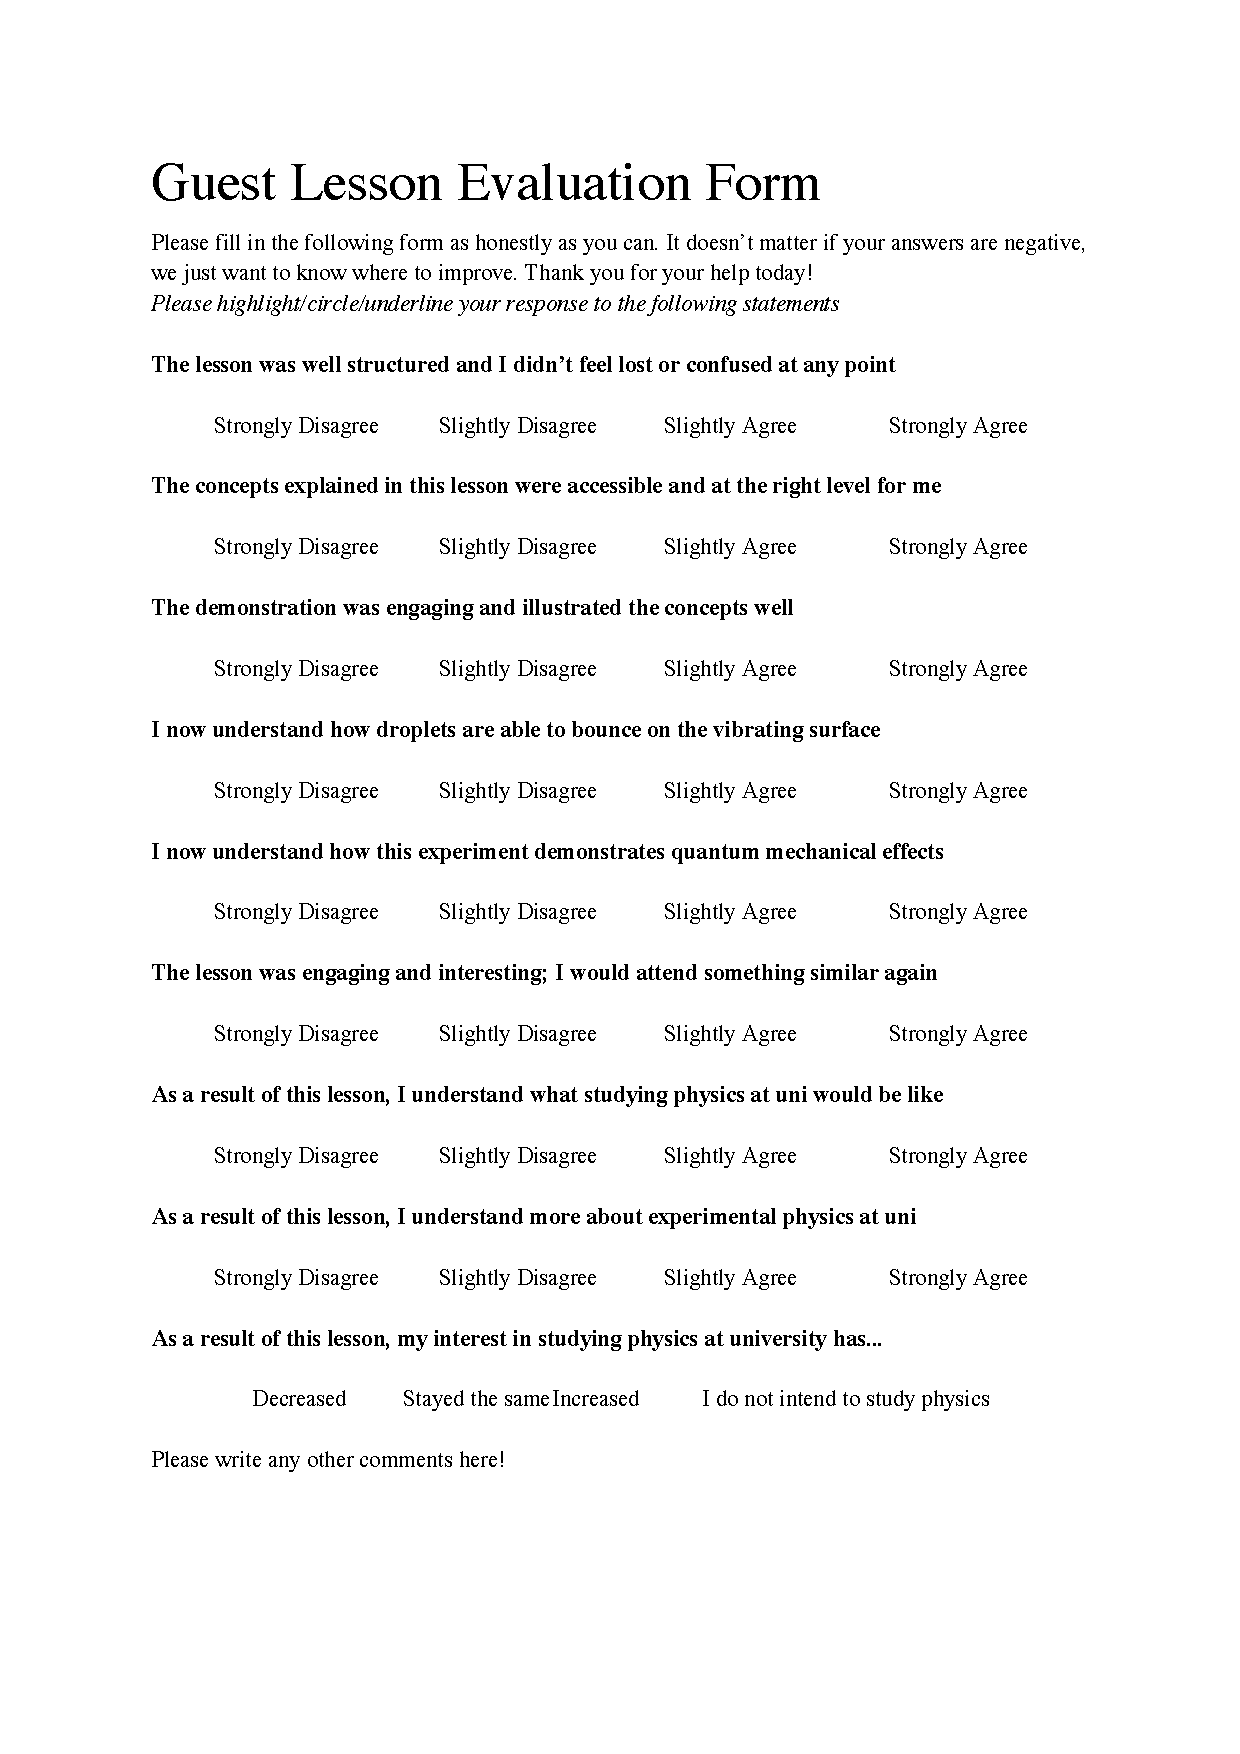
\includepdf{education/evaluation.pdf}
\spacing{1.2}

\bibliographystyle{IEEEtran}
\bibliography{bibliography.bib}

\clearpage
\noindent 
\section{Appendix A: Minutes 11/1/18}

\noindent Meeting Time: 4pm Thursday 11th Jan

\noindent Meeting Location: Massey Group Study Pod, 3rd Floor, Science Library
\\\\
\noindent \textbf{\underbar{Attendance}}

\noindent Chair: Chong Keat Gea CKG

\noindent Vice-Chair: Kelvin Fang KF

\noindent Secretary: Johnny Allain-Labon JAL

\noindent Treasurer: Mohit Motwani MM

\noindent Georges Ajaka GA

\noindent Course Coordinator Point of Contact: Steven Vuong SV

\noindent Benji Berczi BB

\noindent Alex Stock AS

\noindent Prof. Ryan Nichol RN

\noindent 

\noindent Present: CKG KF JAL MM GA SV BB AS RN

\noindent 
\\
\begin{enumerate}
\item  \textbf{Project Outline}

\begin{enumerate}
\item \textbf{ }Existing equipment: none, constructing prototype from scratch

\item  Prototype - start as simple as possible e.g. petri dish on loudspeaker e.g. \url{https://www.youtube.com/watch?v=WIyTZDHuarQ}.  Move on to more complex behaviour if possible

\item  Simulation Programme - want to demonstrate quantum behaviours of the bouncing oil drops if experimental verification is problematic + add missing features of experiment.\\
\end{enumerate}

\item  \textbf{Aims \& Objectives}

\begin{enumerate}
\item \textbf{ }Construct prototype:

\begin{enumerate}
\item  Drop bouncing

\item  Stable drop bouncing over several seconds

\item  Getting the drops to walk

\item  Drop interaction with boundaries

\item  Two or more drops

\item  Drops orbiting

\item  Double slit interference

\item  Tunnelling
\end{enumerate}

\item  Simulation: demonstrate same effects on a computer

\begin{enumerate}
\item  Start with 2D plot

\item  Look to animate with 3D movement
\end{enumerate}

\item  Aim: outreach tool for demonstrating quantum effects on real life scale

\begin{enumerate}
\item  Ideally interactive i.e. can add new droplets

\item  Replicable by teachers
\end{enumerate}

\item  Stretch aim: video demonstrating + different containers/parameters e.g. frequency - bounce to a song?\\
\end{enumerate}

\item  \textbf{Assessment Criteria}

\begin{enumerate}
\item \textbf{ }Working prototype

\item  Working simulation

\item  Reporting\\
\end{enumerate}

\item  \textbf{Deadlines}

\begin{enumerate}
\item \textbf{ }14/1 - Research deadlines - need understanding of scope of project i.e. read papers. Including summary of papers for presentation in formal report. Maintain file ``notes and background reading''

\item  18/1 4pm - Plan for Prototype + Outline for simulation

\item  12/2 - READING WEEK - Basic simulation + prototype completed

\item  Reading Week - report to other group

\item  7/3 - prelim deadline for poster being finalised for printing

\item  16/3 5pm - FINAL REPORT due + critical self-assessment

\item  21/3 - poster presentation\\
\end{enumerate}

\item  \textbf{Areas of Responsibility}

\begin{enumerate}
\item \textbf{ }General Time Management - JAL

\item  Prototype Weds 17/1 6pm brainstorm

\begin{enumerate}
\item  SV Lead

\item  KF

\item  BB

\item  MM

\item  CKG
\end{enumerate}

\item  Simulation - written in Python - Weds 17/1 6pm brainstorm

\begin{enumerate}
\item  GA Lead

\item  AS

\item  JAL
\end{enumerate}

\item  Written Reporting - written as we go - MM\\
\end{enumerate}

\item  \textbf{Communications Plan}

\begin{enumerate}
\item \textbf{ }Google Drive for documents

\item  ShareLatex for written reports

\item  Facebook group for updates, requests for help, anything permanent

\item  FB chat for real time but ephemeral communication\\
\end{enumerate}

\item  \textbf{Future Meetings}

\begin{enumerate}
\item \textbf{ }Thursdays 4pm - regular slot

\item  Thursday 18/1 13:30-14:00 subgroup meeting

\item  Thursday 18/1 16:00 - KF to book

\item  RK availability - to be emailed

\item  Lab use - Derick will accommodate people available, 9-5 lab hours with lunch at 1. Other spaces available for building things - Institute of Making - CKG has one
\end{enumerate}
\end{enumerate}



\spacing{1.2}

\clearpage

\noindent 
\section{Appendix B: Minutes 18/1/18}

\noindent Meeting Time: 4pm Thursday 18th Jan

\noindent Meeting Location: Massey Group Study Pod, 3rd Floor, Science Library\textbf{}\\

\noindent 

\noindent \textbf{\underbar{Attendance}}

\noindent Chair: Chong Keat Gea CKG

\noindent Vice-Chair: Kelvin Fang KF

\noindent Secretary: Johnny Allain-Labon JAL

\noindent Treasurer: Mohit Motwani MM

\noindent Georges Ajaka GA

\noindent Course Coordinator Point of Contact: Steven Vuong SV

\noindent Benji Berczi BB

\noindent Alex Stock AS

\noindent 

\noindent Present: CKG KF JAL MM GA SV BB AS\\

\noindent 

\begin{enumerate}
\item  \textbf{Simulation Group GA}

\begin{enumerate}
\item \textbf{ }How far into the simulation are we?

\begin{enumerate}
\item  3D isn't really possible - only by pre-rendering - takes 5 mins for a pre-rendered version to load

\item  Live-simulation done with heat maps
\end{enumerate}

\item  What can we simulate now?

\begin{enumerate}
\item  Basic animation of wave equation in Python
\end{enumerate}

\item  Have we reached movement?

\begin{enumerate}
\item  Basic movement in Python
\end{enumerate}

\item  Any issues with the coding? 

\begin{enumerate}
\item  Python too slow to render live
\end{enumerate}

\item  Are there sufficient/ too many people working on the code? 

\begin{enumerate}
\item  Don't know yet
\end{enumerate}

\item  Who's done what? Are there any collaboration issues? 

\begin{enumerate}
\item  None yet
\end{enumerate}

\item  Any issues with the code? Buggy, inefficient etc. 

\begin{enumerate}
\item  None to report
\end{enumerate}

\item  What's next? 

\begin{enumerate}
\item  Meeting Monday 11am

\item  Port Python to Java using AWT - JAL

\item  Equations from paper GA AS
\end{enumerate}

\item  Goals setting for next week

\begin{enumerate}
\item  Team GitHub
\end{enumerate}

\item  Who's doing what? 

\item  Discussion with the rest of the team on possible directions and improvements. \\
\end{enumerate}

\item  \textbf{Prototype Group SV}

\begin{enumerate}
\item \textbf{ }How far into the prototype are we? 

\begin{enumerate}
\item  Use Veritasium model as baseline

\item  Have list of materials

\item  Pro-level cameras outside our budget $\mathrm{\to}$ use phones with cameras \& timestamps - issues with timing precision
\end{enumerate}

\item  Propose current idea for apparatus

\begin{enumerate}
\item \url{ https://drive.google.com/drive/folders/1OnPH\_cwJg6xc4uVNFHgWOlpQpYrkzFWK}

\item  Total estimated cost $\mathsterling$80
\end{enumerate}

\item  What equipment do we need, how much will it cost us? Budgeting.

\begin{enumerate}
\item  Camera needs depend on aims - do we want to demonstrate (less hi-spec) or do we want to verify theory (higher-spec)

\item  Use IoM for 3D printing, free wood to use in construction

\item  Light diffuser to illuminate surface + drop more softly

\item  Polarising filter to protect camera?
\end{enumerate}

\item  Possible concerns raised with the equipment and discussion on solution. 

\item  Time frame from getting equipment. When will we get everything and start construction?

\begin{enumerate}
\item  3 working days - can pay more for advanced deliver 

\item  Need equipment by Tuesday 23/1
\end{enumerate}

\item  Any task delegation issues, too many/ not enough people. 

\item  What's next? 

\item  Goal setting for next week? 

\item  Whos doing what? 

\item  Discussion with the rest of the team on possible directions and improvements. 

\begin{enumerate}
\item  Derek - Silicone oil given to us.

\begin{enumerate}
\item  He might have a 50W power supply downstairs

\item  Ask about Amazon Packages
\end{enumerate}

\item  To ask Bernard about: 

\begin{enumerate}
\item  Petri Dish (If not, take from Chemistry / Biology)

\item  50W power supply for Subwoofer

\item  3D Printer
\end{enumerate}

\item  Things to Consider: 

\begin{enumerate}
\item  Diffuser: Need a strong lighting source

\item  LEDs?

\item  Powerful lamps perhaps

\item  Polarising Lens perhaps

\item  IoM, check induction times
\end{enumerate}

\item  Creatables: 

\begin{enumerate}
\item  Lab Script for the entire process\\
\end{enumerate}
\end{enumerate}
\end{enumerate}


\noindent 

\item  \textbf{Written Reporting MM}

\begin{enumerate}
\item \textbf{ }Minutes from last meeting to ShareLatex

\item  Can start writing theory section now - MM to liaise with GA AS JAL\\
\end{enumerate}

\item  \textbf{Project Management JAL}

\begin{enumerate}
\item \textbf{ }Zoho Projects - please confirm login details have been received
\end{enumerate}
\end{enumerate}
\spacing{1.2}

\clearpage
\noindent 
\section{Appendix C: Minutes 25/1/18}

\noindent Meeting Time: 4pm Thursday 25th Jan

\noindent Meeting Location: Group Study Pod 3, Ground Floor, Science Library\textbf{}\\

\noindent 

\noindent \textbf{\underbar{Attendance}}

\noindent Chair: Chong Keat Gea CKG

\noindent Vice-Chair: Kelvin Fang KF

\noindent Secretary: Johnny Allain-Labon JAL

\noindent Treasurer: Mohit Motwani MM

\noindent Georges Ajaka GA

\noindent Course Coordinator Point of Contact: Steven Vuong SV

\noindent Benji Berczi BB

\noindent Alex Stock AS

\noindent Prof Ryan Nichol RN

\noindent 

\noindent Present: CKG KF JAL MM GA SV BB AS

\noindent Absent with Apologies: RN\\

\noindent 

\begin{enumerate}
\item  \textbf{Overall Group Health CKG}

\begin{enumerate}
\item Is everyone ok with what they are working on? (People feeling they aren't contributing enough or doing too much etc.)

\item  Any issues wrt group dynamics etc? No, all going OK.

\end{enumerate}

\item  \textbf{Simulation Group Update GA}

\begin{enumerate}
\item \textbf{ }What has been accomplished in the past week? Were the goals set up last week accomplished? (Last Week Goals: Team github)

\begin{enumerate}
\item  Github permissions are tricky
\end{enumerate}

\item  Request for help: equations to implement in code

\begin{enumerate}
\item  Possible solution would be to square the wave to generate probability of next position and velocity towards next position can be calculated using time stamp (CKG)

\item  GUI written but not running yet - error on compilation

\item  AS - update on equations - need to do integrals by brute force but should work - possibly computationally intensive? And has expected values of coefficients - \url{http://dx.doi.org/10.1063/1.4817612} \url{https://www.cambridge.org/core/journals/journal-of-fluid-mechanics/article/drops-bouncing-on-a-vibrating-bath/441A614F657E800EA06F6C08674CCE67}
\end{enumerate}

\item  Discussion on possible solution

\item  What's next, who does what?

\begin{enumerate}
\item  Implement found equations in Java

\item  Meet Monday to update
\end{enumerate}

\item  Someone to join simulation team eventually?\\
\end{enumerate}

\item  \textbf{Prototype Group Update SV}

\begin{enumerate}
\item \textbf{ }What has been accomplished in the past week? Were the goals set up last week accomplished? (Last Week Goals: ??)

\begin{enumerate}
\item  Got prototype working but droplets too large - due to viscosity? Use different oil with lower viscosity

\item  Smaller droplets accomplished by using a finer point, or using a device to release the drop at a given time
\end{enumerate}

\item  Discussion on the different proposed apparatus. To glue or not to glue?

\begin{enumerate}
\item  Attempt non-permanent options before gluing - double sided tape, 
\end{enumerate}

\item  Any more equipment need purchasing?

\begin{enumerate}
\item  Need to look at other amps - EEng?
\end{enumerate}

\item  What's next, who does what?

\begin{enumerate}
\item  Next Weds for labs

\item  Fix petri dish to speaker - hot glue?

\item  Decide on oil to use - less viscous - CK \& BB

\item  Speaker stand - CK\\
\end{enumerate}
\end{enumerate}

\item  \textbf{Written Reporting Update MM}

\begin{enumerate}
\item \textbf{ }Where are we on this? Do you need help? 

\begin{enumerate}
\item  ShareLatex set up - everyone to test collaboration access please\\
\end{enumerate}
\end{enumerate}

\item  \textbf{AOB}

\begin{enumerate}
\item \textbf{ }Speakers - driven by a signal generator

\item  Can purchase an amplifier if needed - money available in budget - $\mathsterling$125 left
\end{enumerate}
\end{enumerate}





\spacing{1.2}

\clearpage

\noindent 
\section{Appendix D: Minutes 01/2/18}

\noindent Meeting Time: 4pm Thursday 25th Jan

\noindent Meeting Location: First Year Labs\textbf{}\\

\noindent 

\noindent \textbf{\underbar{Attendance}}

\noindent Chair: Chong Keat Gea CKG

\noindent Vice-Chair: Kelvin Fang KF

\noindent Secretary: Johnny Allain-Labon JAL

\noindent Treasurer: Mohit Motwani MM

\noindent Georges Ajaka GA

\noindent Course Coordinator Point of Contact: Steven Vuong SV

\noindent Benji Berczi BB

\noindent Alex Stock AS

\noindent 

\noindent Present: CKG KF JAL MM GA SC BB AS

\noindent Absent with Apologies: \\

\noindent 

\begin{enumerate}
\item  \textbf{Overall Group Health CKG}

\begin{enumerate}
\item \textbf{ }Is everyone ok with what they are working on? (People feeling they aren't contributing enough or doing too much etc.)

\item  Any issues wrt group dynamics etc.

\item  Acknowledgement to team sizing issues. Will be discussed again after the updates from each team.

\begin{enumerate}
\item  Going to wait on update from simulation team to rearrange\\
\end{enumerate}
\end{enumerate}

\item  \textbf{Simulation Group Update GA}

\begin{enumerate}
\item \textbf{ }What has been accomplished in the past week? Were the goals set up last week accomplished? (Implement found equations in Java, Meet Monday to update)

\item  Is the GUI working? Yes, CKG to edit

\item  Have the proposed methods been tested / whats the result? None yet - maths still to be implemented

\item  Any issues to raise? (work allocation, number of people,  math etc.)

\item  What's next? Goal setting for next week

\begin{enumerate}
\item  Improve robustness of simulation

\item  Implement and add new maths

\item  Computing power from UCL requires permission from project supervisor\\
\end{enumerate}
\end{enumerate}

\item  \textbf{Prototype Group Update SV}

\begin{enumerate}
\item \textbf{ }What has been accomplished in the past week? Were the goals set up last week accomplished? (Last Week Goals: Fix petri dish to speaker - hot glue? , Decide on oil to use - less viscous, Speaker stand)

\begin{enumerate}
\item  Cameras have been located to use

\item  Demonstrated multiple bouncing drops \& coupling

\item  Tested in f=50-80Hz

\item  Still need to glue base down
\end{enumerate}

\item  Stage of the prototype?

\item  Any issues to raise (work allocation, number of people, what to test next, etc)

\item  What's next? Goal setting for next week

\begin{enumerate}
\item  Glueing base down

\item  Record droplet in motion

\item  Experiment with amplitudes

\item  Quantify observations

\item  Rest tunnelling\\
\end{enumerate}
\end{enumerate}

\item  \textbf{Written Reporting Update MM}

\begin{enumerate}
\item \textbf{ }Where are we on this? Do you need help?

\begin{enumerate}
\item  No progress without maths and finalised equipment list
\end{enumerate}

\item  Has everyone tested the collab?

\begin{enumerate}
\item  JAL can, assume it generalises\\
\end{enumerate}
\end{enumerate}

\item  \textbf{Team reallocation CKG}

\begin{enumerate}
\item \textbf{ }Discussion on needs of each group.

\begin{enumerate}
\item  BB to start work on poster design, collab w MM for copy
\end{enumerate}

\item  Self evaluation on what each person has contributed and areas for improvement.
\end{enumerate}
\end{enumerate}




\spacing{1.2}

\vspace{\fill}
\section{Appendix E: Powerpoint used in educational outreach}
\includepdf[pages=-]{education/ppt.pdf}


\end{document}